% =====================================================================
%  MANUSCRITO — Revisão Sistemática da Literatura (RSL) — Revista iSys
%  Template oficial: classe SBC (sbc2025.cls) — iSys 2026 "Preferred".
%
%  Tema: Generative AI for Open Government Data Access and Transparency
%
%  >>> ESQUELETO <<<  As seções de resultado/síntese dependem da revisão
%  conduzida (extensão do Mapeamento Sistemático existente) e estão
%  marcadas com  % TODO (depende da revisão conduzida).
%
%  >>> SINGLE-BLIND <<<  O periódico opera revisão single-blind: os AUTORES
%  DEVEM ser identificados no PDF (nome, ORCID, afiliação, e-mail).
%  Preencher os campos marcados com TODO (ORCID/e-mail/afiliação).
%
%  Idioma do corpo: português  ->  classe carregada com [brazilian].
%  O TÍTULO deve estar em inglês, independentemente do idioma do corpo.
%
%  >>> COMPILAR COM XeLaTeX <<<  (exigência do periódico).
%  Pacotes CTAN exigidos pela classe: orcidlink, fontawesome (e, no
%  caminho XeLaTeX, as fontes TeX Gyre Termes e Roboto). Ver CHECKLIST.
% =====================================================================
\documentclass[brazilian]{sbc2025}

\usepackage{aas_macros}
\usepackage[bottom]{footmisc}
\usepackage{afterpage}
\usepackage{url}
\usepackage{pifont}
\usepackage{underscore} % permite "_" em modo texto (DOIs nas referências)

\setcitestyle{square}

% ---- Metadados do periódico (preenchidos pela editoria na publicação) ----
\jid{iSys}
\jtitle{iSys - Journal of Information Systems, 202X, XX:1}
\issn{1984-2902}
\doi{10.5753/isys.202X.XXXXXX}
\copyrightstatement{This work is licensed under a Creative Commons Attribution 4.0 International License}
\jyear{202X}

% TODO: confirmar a categoria correta para uma RSL (ex.: "Review Paper").
\category{Research Paper}

% Título sempre em inglês (exigência da classe). [versão curta opcional]
\title[Generative AI for Open Government Data: An SLR]{Generative AI for Open
Government Data Access and Public Transparency: A Systematic Literature Review}

% --- Autoria identificada (single-blind). \faEnvelopeO = autor correspondente. ---
\author[Oliveira et al. 202X]{
\affil{\textbf{Ana Beatriz Carvalho Oliveira}~\orcidlink{0009-0004-3454-6527}~\textcolor{blue}{\faEnvelopeO}~~[{Universidade Federal de Sergipe}~|\href{mailto:anabeatrizcarvalho@academico.ufs.br}{~{\textit{anabeatrizcarvalho@academico.ufs.br}}}~]}

\affil{\textbf{Gilton José Ferreira da Silva}~\orcidlink{0000-0002-2281-9426}~~[{Universidade Federal de Sergipe}~|\href{mailto:gilton@dcomp.ufs.br}{{\textit{gilton@dcomp.ufs.br}}}~]}
}

\begin{document}

\begin{frontmatter}

\maketitle

\begin{mail}
Departamento de Computação, Universidade Federal de Sergipe, São Cristóvão -- SE, Brasil.
\end{mail}

% ---------------------------------------------------------------------
%  RESUMOS  (Resumo deve ter 200–250 palavras, estruturado, 1 parágrafo)
% ---------------------------------------------------------------------
\begin{abstract-pt}
% TODO (depende da revisão conduzida): atualizar números e achados ao final.
[Contexto] A disponibilização de dados governamentais em formato aberto amplia
o potencial de transparência pública, mas a complexidade e o volume desses
dados impõem barreiras de acesso ao cidadão. [Objetivo] Este artigo investiga
como a Inteligência Artificial Generativa e os \emph{Large Language Models}
(LLMs) vêm sendo aplicados ao acesso a dados governamentais abertos e à
promoção da transparência pública. [Método] Conduziu-se uma Revisão Sistemática
da Literatura segundo as diretrizes de Kitchenham e o reporte PRISMA~2020,
abrangendo bases internacionais e busca por \emph{snowballing}. [Resultados]
\textbf{[TODO: nº de estudos incluídos; principais aplicações; tipos de dados;
LLMs; benefícios; e desafios.]} [Conclusão/Contribuições] A revisão mapeia um
campo emergente na interseção entre governo digital, dados abertos e IA
Generativa, contribuindo para a agenda de pesquisa em Sistemas de Informação.
\end{abstract-pt}

\begin{abstract-en}
[Context] The release of government data in open formats expands the potential
for public transparency, yet the complexity and volume of such data impose
access barriers for citizens. [Objective] This article investigates how
Generative Artificial Intelligence and Large Language Models (LLMs) have been
applied to open government data access and to fostering public transparency.
[Method] We conducted a Systematic Literature Review following Kitchenham's
guidelines and PRISMA~2020 reporting, covering international databases and
snowballing. [Results] \textbf{[TODO: number of included studies; main
applications; data types; LLMs; benefits; and challenges.]}
[Conclusion/Contribution] The review maps an emerging field at the intersection
of digital government, open data, and Generative AI, contributing to the
Information Systems research agenda.
\end{abstract-en}

\begin{pchaves}
IA Generativa, Large Language Models, Dados Governamentais Abertos,
Transparência Pública, Governo Digital, Revisão Sistemática da Literatura
\end{pchaves}

\begin{keywords}
Generative AI, Large Language Models, Open Government Data, Public Transparency,
Digital Government, Systematic Literature Review
\end{keywords}

\begin{dates}
\noindent{\sffamily\textbf{Received:}} DD Month YYYY~~~$\bullet$~~~
{\sffamily\textbf{Accepted:}} DD Month YYYY~~~$\bullet$~~~
{\sffamily\textbf{Published:}} DD Month YYYY
\end{dates}

\end{frontmatter}

% =====================================================================
\section{Introdução}
\label{sec:intro}
% =====================================================================
% Enquadramento EXPLÍCITO em Sistemas de Informação (requisito iSys):
% transparência pública, governo digital, open government data, acesso à
% informação e apoio à decisão. Evitar que pareça apenas "PLN/IA".
% Reuso de enquadramento: capitulos/introducao.tex e capitulos/fundamentacao.tex.

A transparência pública e o acesso à informação são pilares do governo digital
e objeto recorrente de pesquisa em Sistemas de Informação. A disponibilização
de \emph{open government data} (OGD) tem ampliado as bases para
\emph{accountability} e controle social, mas a mera publicação de dados brutos
não garante acesso efetivo: persistem barreiras cognitivas e técnicas entre o
dado e o cidadão.

Embora a literatura de governo digital documente os benefícios da abertura de
dados, e a literatura recente de IA Generativa demonstre avanços na compreensão
e geração de linguagem natural sobre documentos complexos, a interseção entre
ambos — o uso de LLMs para tornar dados governamentais abertos efetivamente
acessíveis e para fortalecer a transparência — permanece fragmentada e carente
de síntese.
% TODO (depende da §2/Background): ancorar este parágrafo com referências de SI
% sobre OGD/e-gov (p.ex., Janssen, Charalabidis, Zuiderwijk, Attard) e de IA
% Generativa (p.ex., Bommasani; Lewis/RAG), e posicionar frente a RSLs prévias.

\paragraph{Objetivo e contribuições.} Este artigo mapeia sistematicamente como a
IA Generativa e os LLMs vêm sendo aplicados ao acesso a dados governamentais
abertos (OGD) e à transparência pública, caracterizando aplicações (RQ1), tipos
de dados (RQ2), modelos (RQ3), benefícios (RQ4) e desafios (RQ5). Dessa
caracterização derivam três contribuições: (i) um panorama do estado da arte;
(ii) uma taxonomia emergente de usos; e (iii) uma agenda de pesquisa para
Sistemas de Informação.

\paragraph{Organização.} A Seção~\ref{sec:background} apresenta o referencial e
os trabalhos relacionados; a Seção~\ref{sec:metodo} detalha o protocolo da
revisão; a Seção~\ref{sec:resultados} reporta os resultados; a
Seção~\ref{sec:discussao} discute as implicações; a Seção~\ref{sec:ameacas}
trata das ameaças à validade; e a Seção~\ref{sec:conclusao} conclui.

% =====================================================================
\section{Background e Trabalhos Relacionados}
\label{sec:background}
% =====================================================================
% Posicionar em venues de Sistemas de Informação: iSys, SBSI, GranDSI-BR,
% MIS Quarterly, Information Systems Research, Decision Support Systems,
% ECIS, ICIS, AMCIS.

\subsection{Dados governamentais abertos e a lacuna de acesso}
\label{subsec:bg_ogd}

\emph{Open government data} (OGD) designa dados produzidos ou custodiados pelo
setor público, disponibilizados em formato legível por máquina e sob licença que
permite reúso \citep{ZuiderwijkJanssen2014}. Em Sistemas de Informação, a agenda
de OGD articula-se às de governo digital e \emph{accountability}: a abertura é
tratada como infraestrutura para o controle social, e não como fim em si
\citep{RibeiroAlmeida2011,OliveiraCkagnazaroff2022}. A literatura, contudo,
distingue de forma consistente \emph{disponibilização} de \emph{uso efetivo}.
Políticas de abertura variam amplamente em implementação e impacto
\citep{ZuiderwijkJanssen2014}, e a qualidade dos dados publicados --- completude,
atualidade, consistência --- com frequência compromete o reúso
\citep{Vetro2016}.

Mesmo com qualidade técnica adequada, persiste uma barreira de outra natureza: a
distância entre o dado bruto e o cidadão capaz de interpretá-lo. Estudos de
interação humano-dados e de literacia de dados mostram que extrair sentido de
conjuntos governamentais exige competências de leitura, consulta e visualização
que não estão uniformemente distribuídas na população
\citep{Hornung2015,Lee2017,Brito2024}. No domínio legislativo, a barreira é
agravada pela natureza dos dados --- textos normativos extensos, com vocabulário
técnico-jurídico e densa referência cruzada --- e pela necessidade de acompanhar
sua evolução ao longo do tempo. É nesse intervalo, entre a publicação e a
compreensão, que se situa o problema de acesso de que trata esta revisão.

\subsection{IA Generativa, LLMs e recuperação aumentada}
\label{subsec:bg_genai}

\emph{Large language models} (LLMs) são modelos treinados sobre grandes volumes
de texto que aprendem a prever e gerar linguagem natural, com desempenho
relevante em sumarização, extração de informação e resposta a perguntas
\citep{JurafskyMartin2023}. Para o acesso a dados governamentais textuais, a
capacidade de interpretar uma consulta em linguagem natural e devolver a resposta
no mesmo registro desloca o ponto de contato do cidadão: em vez de formular
consultas estruturadas ou navegar por portais, ele pergunta diretamente.

Essa promessa esbarra em duas limitações conhecidas. Primeiro, LLMs geram texto
plausível sem garantia de correção factual, produzindo afirmações incorretas
--- \emph{alucinações} ---, especialmente problemáticas num contexto em que a
informação tem efeito normativo \citep{MarquesLaipelt2023}. Segundo, o
conhecimento paramétrico do modelo é estático e desatualiza-se. A geração
aumentada por recuperação (\emph{retrieval-augmented generation}, RAG) responde
a ambos ao condicionar a saída a documentos recuperados em tempo de consulta,
ancorando-a em fontes verificáveis \citep{Lewis2020}. Para dados legislativos,
que mudam e exigem rastreabilidade à fonte, esse condicionamento é menos um
detalhe de implementação do que um requisito.

\subsection{Trabalhos relacionados}
\label{subsec:bg_related}

Tornar dados parlamentares e legislativos acessíveis é tarefa anterior à IA
Generativa. A abordagem predominante até recentemente foi a da Web semântica:
modelar a informação como dados conectados (\emph{Linked Data}) e grafos de
conhecimento, expondo-a por consultas estruturadas
\citep{IsotaniBittencourt2015}. Iniciativas como o ParliamentSampo
\citep{Tamper2022} e o LinkedSaeima \citep{Bojars2019} exemplificam o paradigma:
dados parlamentares ricamente estruturados e interligados, mas acessíveis
sobretudo por consulta formal (por exemplo, SPARQL), o que preserva a barreira
para o usuário não especialista. A IA Generativa propõe deslocar esse paradigma
--- da consulta estruturada para a interação em linguagem natural ---, ao custo
de herdar os problemas de confiabilidade descritos acima.

Apesar do interesse crescente, a interseção entre IA Generativa e acesso a dados
governamentais e legislativos permanece dispersa entre comunidades de pesquisa
--- governo digital, processamento de linguagem natural e Web semântica. Não se
identificou, até a condução desta revisão, um estudo secundário que a sintetize
especificamente, lacuna que justifica a presente RSL e orienta as questões
formuladas na Seção~\ref{sec:metodo}.
% TODO (após a busca): confirmar a ausência de RSL/estudo secundário correlato;
% se algum for recuperado no corpus, posicionar a contribuição explicitamente
% em relação a ele (cobertura, recorte temporal, questões).

% =====================================================================
% Seção de Método completa (protocolo Kitchenham/Charters + PRISMA 2020),
% com tabelas de RQs, PICOC, critérios, qualidade e extração. Reúso do núcleo
% conduzido em capitulos/estado_arte.tex será feito ao redigir os Resultados.
% =====================================================================
%  SEÇÃO DE MÉTODO — Revisão Sistemática da Literatura (RSL)
%  Inserida em isys_rsl.tex via  % =====================================================================
%  SEÇÃO DE MÉTODO — Revisão Sistemática da Literatura (RSL)
%  Inserida em isys_rsl.tex via  % =====================================================================
%  SEÇÃO DE MÉTODO — Revisão Sistemática da Literatura (RSL)
%  Inserida em isys_rsl.tex via  \input{metodo_rsl}
%
%  CLASSE: sbc2025 (apalike-sol). Sem comandos ABNT (\quadro, \citeonline).
%  PACOTES: usa apenas tabular/\hline padrão — não exige booktabs.
%
%  PARÂMETROS A CONFIRMAR (procure por "CONFIRMAR" abaixo):
%   - Janela temporal (ano inicial)
%   - String final após calibração-piloto
%   - Limiares de qualidade
%
%  REFERÊNCIAS .bib:
%   NOVAS (adicionadas a referencias.bib): kitchenham2007, petersen2015,
%         page2021, wohlin2014.
%   NOTA: Kitchenham2004 (mapeamento) já existe no .bib, mas é obra distinta;
%         o Método cita Kitchenham & Charters (2007) = kitchenham2007.
%
%  OBS.: se a classe for de duas colunas e alguma tabela estourar,
%        troque \begin{table} por \begin{table*}.
% =====================================================================

\section{Método}
\label{sec:metodo}

Este trabalho caracteriza-se como uma Revisão Sistemática da Literatura (RSL), método secundário cujo propósito é identificar, avaliar e sintetizar as evidências científicas disponíveis sobre um dado fenômeno de forma reprozível. O protocolo foi planejado e conduzido segundo as diretrizes de Kitchenham e Charters \citeyearpar{kitchenham2007}, complementadas pelas orientações para mapeamento sistemático de Petersen et al. \citeyearpar{petersen2015}. O relato da pesquisa obedece às recomendações do framework PRISMA 2020 \citep{page2021}.

Como as questões levantadas são de caracterização, e não explicativas, optou-se por um desenho \textbf{híbrido}. Isso significa que a busca e a seleção de literatura seguem o rigor procedimental de uma RSL, mas a síntese dos resultados assume a abrangência de um mapeamento de campo. A execução organiza-se em três etapas: planejamento (definição do protocolo e critérios), condução (busca, seleção e extração) e relato (síntese e discussão). Visando proteger a reprodutibilidade do estudo e refrear o viés do pesquisador, todo o protocolo foi consolidado \textit{a priori}.

\subsection{Objetivo e Questões de Pesquisa}
\label{subsec:objetivo_qp}

O objetivo desta revisão é identificar como a Inteligência Artificial Generativa e os Modelos de Linguagem de Grande Porte (\textit{Large Language Models} -- LLMs) vêm sendo empregados para destravar o acesso a dados governamentais abertos e impulsionar a transparência pública. O esforço ancora-se na área de Sistemas de Informação, operando exatamente na interseção entre governo digital, política de dados abertos (\textit{Open Government Data} -- OGD) e apoio à decisão. A partir dessa diretriz central, derivam-se as cinco questões de pesquisa detalhadas na Tabela~\ref{tab:rqs}.

\begin{table*}[t]
\centering
\caption{Questões de pesquisa e foco de extração}
\label{tab:rqs}
\small
\begin{tabular}{|c|p{4.6cm}|p{4.0cm}|}
\hline
\textbf{ID} & \textbf{Questão de pesquisa} & \textbf{Foco da extração} \\ \hline
RQ1 & Quais aplicações de IA Generativa são utilizadas no acesso a dados governamentais abertos e na transparência pública? & Tipo de aplicação / caso de uso \\ \hline
RQ2 & Quais tipos de dados governamentais são analisados? & Natureza e domínio dos dados \\ \hline
RQ3 & Quais LLMs são utilizados? & Modelo(s), porte, aberto/proprietário \\ \hline
RQ4 & Quais benefícios são reportados? & Ganhos de acesso e transparência \\ \hline
RQ5 & Quais desafios e limitações são reportados? & Barreiras técnicas, éticas e de adoção \\ \hline
\end{tabular}
\end{table*}

\subsection{Estratégia de Busca}
\label{subsec:busca}

A varredura automática ocorreu em quatro bases de amplo reconhecimento no domínio da Computação: Scopus, Web of Science, ACM Digital Library e IEEE Xplore. Essa seleção equilibra indexadores multidisciplinares (Scopus, WoS) e repositórios de nicho tecnológico (ACM, IEEE), mitigando o risco de omissão de publicações chave.

Os termos da consulta foram arquitetados a partir das cinco dimensões da estrutura PICOC (Tabela~\ref{tab:picoc}), garantindo que a \textit{string} não recaísse isoladamente sobre a Intervenção tecnológica. O eixo de Intervenção mapeia o maquinário propriamente dito: IA Generativa, modelos de fundação, \textit{transformers}, arquiteturas RAG, agentes conversacionais e LLMs comerciais ou abertos. Em contrapartida, os blocos de População, Desfecho e Contexto amarram o escopo da ferramenta ao setor público, filtrando estritamente estudos sobre portais governamentais, dados legislativos e políticas de transparência digital.

A \textit{string} de referência consta na Figura~\ref{fig:string} e foi adaptada às regras sintáticas de cada base no momento do disparo. Para assegurar aderência ao critério de idioma (CI4), aplicou-se uma variação do comando em português à Biblioteca Digital da SBC/SOL e demais plataformas lusófonas. Com o intuito de distinguir a real escassez de produção acadêmica de meros erros de digitação na busca, a estrutura sintática exata, a data e o volume retornado por base foram documentados no repositório do projeto e recuperados na Seção~\ref{sec:resultados}.

\begin{table*}[t]
\centering
\caption{Termos da busca segundo a estrutura PICOC}
\label{tab:picoc}
\small
\begin{tabular}{|p{2.4cm}|p{6.0cm}|}
\hline
\textbf{Elemento} & \textbf{Termos} \\ \hline
População & Setor público; portais e dados governamentais \\ \hline
Intervenção & IA Generativa; LLMs; modelos de linguagem \\ \hline
Comparação & Não aplicável (revisão de caracterização) \\ \hline
Desfecho & Acesso à informação; transparência; benefícios e desafios \\ \hline
Contexto & Governo digital; \textit{e-government}; OGD \\ \hline
\end{tabular}
\end{table*}

\begin{figure*}[t]
\centering
\begin{minipage}{0.95\textwidth}
\begin{small}
\begin{verbatim}
("generative artificial intelligence" OR "generative AI"
 OR "large language model*" OR "LLM*" OR "foundation model*"
 OR transformer* OR GPT* OR ChatGPT OR Llama OR Mistral OR Gemini
 OR "retrieval-augmented generation" OR RAG
 OR chatbot* OR "conversational agent*")
AND
("open government data" OR "open data" OR "government data"
 OR "public sector data" OR "legislative data" OR "parliamentary data"
 OR "freedom of information" OR FOIA OR "access to information"
 OR transparency OR accountability
 OR "digital government" OR "e-government" OR "open government"
 OR "data portal*")
\end{verbatim}
\end{small}
\end{minipage}
\caption{String de busca de referência, com dois blocos conectados por \texttt{AND}: o primeiro reúne termos de IA Generativa/LLMs (Intervenção); o segundo, termos de dados governamentais abertos, governo digital e transparência (População, Desfecho, Contexto). A sintaxe é adaptada a cada base no momento da execução.}
\label{fig:string}
\end{figure*}

Antes da execução definitiva, a \textit{string} passou por calibração-piloto. Ela foi confrontada contra um acervo de controle previamente mapeado pela literatura: caso algum desses artigos essenciais não fosse detectado, o escopo de palavras-chave sofreria expansão imediata. % CONFIRMAR: liste 3-5 artigos de controle usados na calibração.

O intervalo temporal abrange de janeiro de 2019 até a data da pesquisa. % CONFIRMAR ano inicial.
A justificativa para o corte repousa no fato de a consolidação dos grandes modelos pré-treinados ter ocorrido sistematicamente a partir de 2019. O esforço apoiou-se exclusivamente no retorno das bases de dados; técnicas auxiliares de prospecção referencial em cascata (\textit{snowballing} para frente e para trás) \citep{wohlin2014} não foram acionadas neste estágio, configurando uma limitação metodológica discutida com maior profundidade na Seção~\ref{sec:ameacas}.

\subsection{Critérios de Seleção e Processo de Triagem}
\label{subsec:selecao}

O filtro do \textit{corpus} bibliográfico baseou-se nos parâmetros expostos na Tabela~\ref{tab:criterios}. O protocolo é excludente: a aprovação final de um artigo exige a conformidade simultânea a todos os critérios de inclusão e a imunidade absoluta a qualquer um dos critérios de exclusão.

\begin{table}[ht]
\centering
\caption{Critérios de inclusão e exclusão}
\label{tab:criterios}
\small
\begin{tabular}{|c|p{6.4cm}|}
\hline
\textbf{ID} & \textbf{Critério} \\ \hline
CI1 & Aplica ou investiga IA Generativa/LLMs em contexto de dados abertos, transparência pública ou governo digital \\ \hline
CI2 & Estudo primário revisado por pares (conferência ou periódico) \\ \hline
CI3 & Publicado na janela temporal definida \\ \hline
CI4 & Texto em inglês ou português \\ \hline
CI5 & Texto completo acessível \\ \hline
CE1 & Aborda apenas um dos eixos (somente IA \textit{ou} somente governo aberto), sem a interseção \\ \hline
CE2 & Estudo secundário (outra revisão, mapeamento ou \textit{survey}) -- considerado apenas como referência para trabalhos relacionados \\ \hline
CE3 & Literatura cinza, editorial, resumo estendido, pôster, \textit{keynote} ou tutorial \\ \hline
CE4 & Duplicata \\ \hline
CE5 & Versão preliminar de estudo posteriormente estendido (mantém-se a versão mais completa) \\ \hline
\end{tabular}
\end{table}

O funil de seleção operou em duas etapas. A triagem inicial ocorreu por meio da leitura rápida de títulos e resumos. Em seguida, os trabalhos pré-selecionados avançaram para a avaliação na íntegra. Todo o referencial foi exportado para o Zotero (responsável pela deduplicação primária) e posteriormente importado para a plataforma Rayyan, onde ocorreu a triagem manual.

Uma única pesquisadora conduziu a revisão. Para mitigar o viés interpretativo individual, todos os parâmetros de inclusão e exclusão foram engessados formalmente no projeto de pesquisa. Além disso, as exclusões no Rayyan exigiram a marcação explícita do rótulo motivador correspondente ao critério CE, gerando uma trilha de auditoria rastreável. O diagrama PRISMA, ilustrado na seção de resultados, consolida todo o fluxo das exclusões.

\subsection{Avaliação de Qualidade}
\label{subsec:qualidade}

Os manuscritos sobreviventes à leitura integral foram então submetidos a um crivo de qualidade focado no rigor científico das evidências. Cada métrica da Tabela~\ref{tab:qualidade} comporta três valores possíveis: $0$ (não atende), $0{,}5$ (atende parcialmente) e $1$ (atende plenamente), culminando em uma pontuação máxima de 5.

Estabeleceu-se o limiar de $2{,}5$ como nota de corte analítica. Trabalhos que igualam ou superam essa barreira compõem o núcleo da síntese informacional sem ressalvas. Aqueles com desempenho inferior não sofrem descarte sumário, mas são apartados em um bloco interpretativo paralelo, exigindo ceticismo deliberado na fase de Discussão.

Esse recurso avaliativo opera também como mecanismo compensatório para publicações em veículos de menor tradição editorial (como simpósios de iniciação ou anais de triagem branda). Pelo critério CI2, estudos primários em eventos oficiais não são descartados na fase inicial. É a matriz de qualidade (notadamente os fatores AQ4 e AQ5) que penaliza a fragilidade argumentativa dessas produções, desidratando sua influência na conclusão final sem violar as regras da filtragem sistemática.

\begin{table}[ht]
\centering
\caption{Critérios de avaliação de qualidade}
\label{tab:qualidade}
\small
\begin{tabular}{|c|p{6.4cm}|}
\hline
\textbf{ID} & \textbf{Critério} \\ \hline
AQ1 & Os objetivos do estudo estão claramente declarados? \\ \hline
AQ2 & O contexto (domínio governamental e dados) está adequadamente descrito? \\ \hline
AQ3 & A abordagem de IA Generativa/LLM está descrita com detalhe suficiente para ser compreendida e replicada? \\ \hline
AQ4 & Os resultados e benefícios são reportados e sustentados por evidências? \\ \hline
AQ5 & As limitações e ameaças à validade são discutidas? \\ \hline
\end{tabular}
\end{table}

\subsection{Extração de Dados}
\label{subsec:extracao}

A captação de evidências seguiu um formulário rígido cujas entradas convergem diretamente para as cinco questões de pesquisa (Tabela~\ref{tab:extracao}). Como complemento à estruturação técnica, levantou-se o inventário bibliométrico padrão (autoria, ano, país e tipologia do veículo), bem como as matrizes metodológicas de validação presentes em cada artigo empírico. Todo o registro das abstrações foi conduzido pela revisora primária, mantendo a indexação rigorosa da informação recolhida com o arquivo de origem para evitar distorções de interpretação fora de contexto.

\begin{table*}[t]
\centering
\caption{Formulário de extração e vínculo com as questões de pesquisa}
\label{tab:extracao}
\small
\renewcommand{\arraystretch}{1.15}
\begin{tabular}{|p{3.6cm}|@{\hspace{0.6em}}p{6.0cm}@{\hspace{0.6em}}|c|}
\hline
\textbf{Campo} & \textbf{Descrição} & \textbf{RQ} \\ \hline
Aplicação / caso de uso & Como a IA Generativa é empregada & RQ1 \\ \hline
Dados governamentais & Tipo e domínio dos dados analisados & RQ2 \\ \hline
Modelo(s) & LLM/IA Generativa, porte, licença & RQ3 \\ \hline
Benefícios & Ganhos de acesso/transparência relatados & RQ4 \\ \hline
Desafios & Limitações técnicas, éticas e de adoção & RQ5 \\ \hline
Avaliação & Método de validação do estudo & --- \\ \hline
\end{tabular}
\end{table*}

\subsection{Síntese dos Dados}
\label{subsec:sintese}

O fechamento da revisão opera sob uma matriz dual. O primeiro pilar baseia-se na \textit{síntese quantitativa descritiva}, responsável por traduzir o volume documental em distribuições macro (como a linha do tempo de publicações, os LLMs mais citados em RQ3 e o espectro de dados analisados em RQ2). O segundo pilar é a \textit{síntese temática}, uma abordagem estritamente qualitativa. Nela, o esforço debruça-se sobre a codificação do texto bruto, extraindo e categorizando de forma orgânica as rotinas governamentais criadas (RQ1), os impactos sociais alcançados (RQ4) e as pedras de tropeço da adoção (RQ5). É o atrito analítico provocado pelo cruzamento dessas duas sínteses que permitirá, no momento da Discussão, organizar o caos de aplicações cívicas de Inteligência Artificial em uma taxonomia coesa e útil para a comunidade científica.

%
%  CLASSE: sbc2025 (apalike-sol). Sem comandos ABNT (\quadro, \citeonline).
%  PACOTES: usa apenas tabular/\hline padrão — não exige booktabs.
%
%  PARÂMETROS A CONFIRMAR (procure por "CONFIRMAR" abaixo):
%   - Janela temporal (ano inicial)
%   - String final após calibração-piloto
%   - Limiares de qualidade
%
%  REFERÊNCIAS .bib:
%   NOVAS (adicionadas a referencias.bib): kitchenham2007, petersen2015,
%         page2021, wohlin2014.
%   NOTA: Kitchenham2004 (mapeamento) já existe no .bib, mas é obra distinta;
%         o Método cita Kitchenham & Charters (2007) = kitchenham2007.
%
%  OBS.: se a classe for de duas colunas e alguma tabela estourar,
%        troque \begin{table} por \begin{table*}.
% =====================================================================

\section{Método}
\label{sec:metodo}

Este trabalho caracteriza-se como uma Revisão Sistemática da Literatura (RSL), método secundário cujo propósito é identificar, avaliar e sintetizar as evidências científicas disponíveis sobre um dado fenômeno de forma reprozível. O protocolo foi planejado e conduzido segundo as diretrizes de Kitchenham e Charters \citeyearpar{kitchenham2007}, complementadas pelas orientações para mapeamento sistemático de Petersen et al. \citeyearpar{petersen2015}. O relato da pesquisa obedece às recomendações do framework PRISMA 2020 \citep{page2021}.

Como as questões levantadas são de caracterização, e não explicativas, optou-se por um desenho \textbf{híbrido}. Isso significa que a busca e a seleção de literatura seguem o rigor procedimental de uma RSL, mas a síntese dos resultados assume a abrangência de um mapeamento de campo. A execução organiza-se em três etapas: planejamento (definição do protocolo e critérios), condução (busca, seleção e extração) e relato (síntese e discussão). Visando proteger a reprodutibilidade do estudo e refrear o viés do pesquisador, todo o protocolo foi consolidado \textit{a priori}.

\subsection{Objetivo e Questões de Pesquisa}
\label{subsec:objetivo_qp}

O objetivo desta revisão é identificar como a Inteligência Artificial Generativa e os Modelos de Linguagem de Grande Porte (\textit{Large Language Models} -- LLMs) vêm sendo empregados para destravar o acesso a dados governamentais abertos e impulsionar a transparência pública. O esforço ancora-se na área de Sistemas de Informação, operando exatamente na interseção entre governo digital, política de dados abertos (\textit{Open Government Data} -- OGD) e apoio à decisão. A partir dessa diretriz central, derivam-se as cinco questões de pesquisa detalhadas na Tabela~\ref{tab:rqs}.

\begin{table*}[t]
\centering
\caption{Questões de pesquisa e foco de extração}
\label{tab:rqs}
\small
\begin{tabular}{|c|p{4.6cm}|p{4.0cm}|}
\hline
\textbf{ID} & \textbf{Questão de pesquisa} & \textbf{Foco da extração} \\ \hline
RQ1 & Quais aplicações de IA Generativa são utilizadas no acesso a dados governamentais abertos e na transparência pública? & Tipo de aplicação / caso de uso \\ \hline
RQ2 & Quais tipos de dados governamentais são analisados? & Natureza e domínio dos dados \\ \hline
RQ3 & Quais LLMs são utilizados? & Modelo(s), porte, aberto/proprietário \\ \hline
RQ4 & Quais benefícios são reportados? & Ganhos de acesso e transparência \\ \hline
RQ5 & Quais desafios e limitações são reportados? & Barreiras técnicas, éticas e de adoção \\ \hline
\end{tabular}
\end{table*}

\subsection{Estratégia de Busca}
\label{subsec:busca}

A varredura automática ocorreu em quatro bases de amplo reconhecimento no domínio da Computação: Scopus, Web of Science, ACM Digital Library e IEEE Xplore. Essa seleção equilibra indexadores multidisciplinares (Scopus, WoS) e repositórios de nicho tecnológico (ACM, IEEE), mitigando o risco de omissão de publicações chave.

Os termos da consulta foram arquitetados a partir das cinco dimensões da estrutura PICOC (Tabela~\ref{tab:picoc}), garantindo que a \textit{string} não recaísse isoladamente sobre a Intervenção tecnológica. O eixo de Intervenção mapeia o maquinário propriamente dito: IA Generativa, modelos de fundação, \textit{transformers}, arquiteturas RAG, agentes conversacionais e LLMs comerciais ou abertos. Em contrapartida, os blocos de População, Desfecho e Contexto amarram o escopo da ferramenta ao setor público, filtrando estritamente estudos sobre portais governamentais, dados legislativos e políticas de transparência digital.

A \textit{string} de referência consta na Figura~\ref{fig:string} e foi adaptada às regras sintáticas de cada base no momento do disparo. Para assegurar aderência ao critério de idioma (CI4), aplicou-se uma variação do comando em português à Biblioteca Digital da SBC/SOL e demais plataformas lusófonas. Com o intuito de distinguir a real escassez de produção acadêmica de meros erros de digitação na busca, a estrutura sintática exata, a data e o volume retornado por base foram documentados no repositório do projeto e recuperados na Seção~\ref{sec:resultados}.

\begin{table*}[t]
\centering
\caption{Termos da busca segundo a estrutura PICOC}
\label{tab:picoc}
\small
\begin{tabular}{|p{2.4cm}|p{6.0cm}|}
\hline
\textbf{Elemento} & \textbf{Termos} \\ \hline
População & Setor público; portais e dados governamentais \\ \hline
Intervenção & IA Generativa; LLMs; modelos de linguagem \\ \hline
Comparação & Não aplicável (revisão de caracterização) \\ \hline
Desfecho & Acesso à informação; transparência; benefícios e desafios \\ \hline
Contexto & Governo digital; \textit{e-government}; OGD \\ \hline
\end{tabular}
\end{table*}

\begin{figure*}[t]
\centering
\begin{minipage}{0.95\textwidth}
\begin{small}
\begin{verbatim}
("generative artificial intelligence" OR "generative AI"
 OR "large language model*" OR "LLM*" OR "foundation model*"
 OR transformer* OR GPT* OR ChatGPT OR Llama OR Mistral OR Gemini
 OR "retrieval-augmented generation" OR RAG
 OR chatbot* OR "conversational agent*")
AND
("open government data" OR "open data" OR "government data"
 OR "public sector data" OR "legislative data" OR "parliamentary data"
 OR "freedom of information" OR FOIA OR "access to information"
 OR transparency OR accountability
 OR "digital government" OR "e-government" OR "open government"
 OR "data portal*")
\end{verbatim}
\end{small}
\end{minipage}
\caption{String de busca de referência, com dois blocos conectados por \texttt{AND}: o primeiro reúne termos de IA Generativa/LLMs (Intervenção); o segundo, termos de dados governamentais abertos, governo digital e transparência (População, Desfecho, Contexto). A sintaxe é adaptada a cada base no momento da execução.}
\label{fig:string}
\end{figure*}

Antes da execução definitiva, a \textit{string} passou por calibração-piloto. Ela foi confrontada contra um acervo de controle previamente mapeado pela literatura: caso algum desses artigos essenciais não fosse detectado, o escopo de palavras-chave sofreria expansão imediata. % CONFIRMAR: liste 3-5 artigos de controle usados na calibração.

O intervalo temporal abrange de janeiro de 2019 até a data da pesquisa. % CONFIRMAR ano inicial.
A justificativa para o corte repousa no fato de a consolidação dos grandes modelos pré-treinados ter ocorrido sistematicamente a partir de 2019. O esforço apoiou-se exclusivamente no retorno das bases de dados; técnicas auxiliares de prospecção referencial em cascata (\textit{snowballing} para frente e para trás) \citep{wohlin2014} não foram acionadas neste estágio, configurando uma limitação metodológica discutida com maior profundidade na Seção~\ref{sec:ameacas}.

\subsection{Critérios de Seleção e Processo de Triagem}
\label{subsec:selecao}

O filtro do \textit{corpus} bibliográfico baseou-se nos parâmetros expostos na Tabela~\ref{tab:criterios}. O protocolo é excludente: a aprovação final de um artigo exige a conformidade simultânea a todos os critérios de inclusão e a imunidade absoluta a qualquer um dos critérios de exclusão.

\begin{table}[ht]
\centering
\caption{Critérios de inclusão e exclusão}
\label{tab:criterios}
\small
\begin{tabular}{|c|p{6.4cm}|}
\hline
\textbf{ID} & \textbf{Critério} \\ \hline
CI1 & Aplica ou investiga IA Generativa/LLMs em contexto de dados abertos, transparência pública ou governo digital \\ \hline
CI2 & Estudo primário revisado por pares (conferência ou periódico) \\ \hline
CI3 & Publicado na janela temporal definida \\ \hline
CI4 & Texto em inglês ou português \\ \hline
CI5 & Texto completo acessível \\ \hline
CE1 & Aborda apenas um dos eixos (somente IA \textit{ou} somente governo aberto), sem a interseção \\ \hline
CE2 & Estudo secundário (outra revisão, mapeamento ou \textit{survey}) -- considerado apenas como referência para trabalhos relacionados \\ \hline
CE3 & Literatura cinza, editorial, resumo estendido, pôster, \textit{keynote} ou tutorial \\ \hline
CE4 & Duplicata \\ \hline
CE5 & Versão preliminar de estudo posteriormente estendido (mantém-se a versão mais completa) \\ \hline
\end{tabular}
\end{table}

O funil de seleção operou em duas etapas. A triagem inicial ocorreu por meio da leitura rápida de títulos e resumos. Em seguida, os trabalhos pré-selecionados avançaram para a avaliação na íntegra. Todo o referencial foi exportado para o Zotero (responsável pela deduplicação primária) e posteriormente importado para a plataforma Rayyan, onde ocorreu a triagem manual.

Uma única pesquisadora conduziu a revisão. Para mitigar o viés interpretativo individual, todos os parâmetros de inclusão e exclusão foram engessados formalmente no projeto de pesquisa. Além disso, as exclusões no Rayyan exigiram a marcação explícita do rótulo motivador correspondente ao critério CE, gerando uma trilha de auditoria rastreável. O diagrama PRISMA, ilustrado na seção de resultados, consolida todo o fluxo das exclusões.

\subsection{Avaliação de Qualidade}
\label{subsec:qualidade}

Os manuscritos sobreviventes à leitura integral foram então submetidos a um crivo de qualidade focado no rigor científico das evidências. Cada métrica da Tabela~\ref{tab:qualidade} comporta três valores possíveis: $0$ (não atende), $0{,}5$ (atende parcialmente) e $1$ (atende plenamente), culminando em uma pontuação máxima de 5.

Estabeleceu-se o limiar de $2{,}5$ como nota de corte analítica. Trabalhos que igualam ou superam essa barreira compõem o núcleo da síntese informacional sem ressalvas. Aqueles com desempenho inferior não sofrem descarte sumário, mas são apartados em um bloco interpretativo paralelo, exigindo ceticismo deliberado na fase de Discussão.

Esse recurso avaliativo opera também como mecanismo compensatório para publicações em veículos de menor tradição editorial (como simpósios de iniciação ou anais de triagem branda). Pelo critério CI2, estudos primários em eventos oficiais não são descartados na fase inicial. É a matriz de qualidade (notadamente os fatores AQ4 e AQ5) que penaliza a fragilidade argumentativa dessas produções, desidratando sua influência na conclusão final sem violar as regras da filtragem sistemática.

\begin{table}[ht]
\centering
\caption{Critérios de avaliação de qualidade}
\label{tab:qualidade}
\small
\begin{tabular}{|c|p{6.4cm}|}
\hline
\textbf{ID} & \textbf{Critério} \\ \hline
AQ1 & Os objetivos do estudo estão claramente declarados? \\ \hline
AQ2 & O contexto (domínio governamental e dados) está adequadamente descrito? \\ \hline
AQ3 & A abordagem de IA Generativa/LLM está descrita com detalhe suficiente para ser compreendida e replicada? \\ \hline
AQ4 & Os resultados e benefícios são reportados e sustentados por evidências? \\ \hline
AQ5 & As limitações e ameaças à validade são discutidas? \\ \hline
\end{tabular}
\end{table}

\subsection{Extração de Dados}
\label{subsec:extracao}

A captação de evidências seguiu um formulário rígido cujas entradas convergem diretamente para as cinco questões de pesquisa (Tabela~\ref{tab:extracao}). Como complemento à estruturação técnica, levantou-se o inventário bibliométrico padrão (autoria, ano, país e tipologia do veículo), bem como as matrizes metodológicas de validação presentes em cada artigo empírico. Todo o registro das abstrações foi conduzido pela revisora primária, mantendo a indexação rigorosa da informação recolhida com o arquivo de origem para evitar distorções de interpretação fora de contexto.

\begin{table*}[t]
\centering
\caption{Formulário de extração e vínculo com as questões de pesquisa}
\label{tab:extracao}
\small
\renewcommand{\arraystretch}{1.15}
\begin{tabular}{|p{3.6cm}|@{\hspace{0.6em}}p{6.0cm}@{\hspace{0.6em}}|c|}
\hline
\textbf{Campo} & \textbf{Descrição} & \textbf{RQ} \\ \hline
Aplicação / caso de uso & Como a IA Generativa é empregada & RQ1 \\ \hline
Dados governamentais & Tipo e domínio dos dados analisados & RQ2 \\ \hline
Modelo(s) & LLM/IA Generativa, porte, licença & RQ3 \\ \hline
Benefícios & Ganhos de acesso/transparência relatados & RQ4 \\ \hline
Desafios & Limitações técnicas, éticas e de adoção & RQ5 \\ \hline
Avaliação & Método de validação do estudo & --- \\ \hline
\end{tabular}
\end{table*}

\subsection{Síntese dos Dados}
\label{subsec:sintese}

O fechamento da revisão opera sob uma matriz dual. O primeiro pilar baseia-se na \textit{síntese quantitativa descritiva}, responsável por traduzir o volume documental em distribuições macro (como a linha do tempo de publicações, os LLMs mais citados em RQ3 e o espectro de dados analisados em RQ2). O segundo pilar é a \textit{síntese temática}, uma abordagem estritamente qualitativa. Nela, o esforço debruça-se sobre a codificação do texto bruto, extraindo e categorizando de forma orgânica as rotinas governamentais criadas (RQ1), os impactos sociais alcançados (RQ4) e as pedras de tropeço da adoção (RQ5). É o atrito analítico provocado pelo cruzamento dessas duas sínteses que permitirá, no momento da Discussão, organizar o caos de aplicações cívicas de Inteligência Artificial em uma taxonomia coesa e útil para a comunidade científica.

%
%  CLASSE: sbc2025 (apalike-sol). Sem comandos ABNT (\quadro, \citeonline).
%  PACOTES: usa apenas tabular/\hline padrão — não exige booktabs.
%
%  PARÂMETROS A CONFIRMAR (procure por "CONFIRMAR" abaixo):
%   - Janela temporal (ano inicial)
%   - String final após calibração-piloto
%   - Limiares de qualidade
%
%  REFERÊNCIAS .bib:
%   NOVAS (adicionadas a referencias.bib): kitchenham2007, petersen2015,
%         page2021, wohlin2014.
%   NOTA: Kitchenham2004 (mapeamento) já existe no .bib, mas é obra distinta;
%         o Método cita Kitchenham & Charters (2007) = kitchenham2007.
%
%  OBS.: se a classe for de duas colunas e alguma tabela estourar,
%        troque \begin{table} por \begin{table*}.
% =====================================================================

\section{Método}
\label{sec:metodo}

Este trabalho caracteriza-se como uma Revisão Sistemática da Literatura (RSL), método secundário cujo propósito é identificar, avaliar e sintetizar as evidências científicas disponíveis sobre um dado fenômeno de forma reprozível. O protocolo foi planejado e conduzido segundo as diretrizes de Kitchenham e Charters \citeyearpar{kitchenham2007}, complementadas pelas orientações para mapeamento sistemático de Petersen et al. \citeyearpar{petersen2015}. O relato da pesquisa obedece às recomendações do framework PRISMA 2020 \citep{page2021}.

Como as questões levantadas são de caracterização, e não explicativas, optou-se por um desenho \textbf{híbrido}. Isso significa que a busca e a seleção de literatura seguem o rigor procedimental de uma RSL, mas a síntese dos resultados assume a abrangência de um mapeamento de campo. A execução organiza-se em três etapas: planejamento (definição do protocolo e critérios), condução (busca, seleção e extração) e relato (síntese e discussão). Visando proteger a reprodutibilidade do estudo e refrear o viés do pesquisador, todo o protocolo foi consolidado \textit{a priori}.

\subsection{Objetivo e Questões de Pesquisa}
\label{subsec:objetivo_qp}

O objetivo desta revisão é identificar como a Inteligência Artificial Generativa e os Modelos de Linguagem de Grande Porte (\textit{Large Language Models} -- LLMs) vêm sendo empregados para destravar o acesso a dados governamentais abertos e impulsionar a transparência pública. O esforço ancora-se na área de Sistemas de Informação, operando exatamente na interseção entre governo digital, política de dados abertos (\textit{Open Government Data} -- OGD) e apoio à decisão. A partir dessa diretriz central, derivam-se as cinco questões de pesquisa detalhadas na Tabela~\ref{tab:rqs}.

\begin{table*}[t]
\centering
\caption{Questões de pesquisa e foco de extração}
\label{tab:rqs}
\small
\begin{tabular}{|c|p{4.6cm}|p{4.0cm}|}
\hline
\textbf{ID} & \textbf{Questão de pesquisa} & \textbf{Foco da extração} \\ \hline
RQ1 & Quais aplicações de IA Generativa são utilizadas no acesso a dados governamentais abertos e na transparência pública? & Tipo de aplicação / caso de uso \\ \hline
RQ2 & Quais tipos de dados governamentais são analisados? & Natureza e domínio dos dados \\ \hline
RQ3 & Quais LLMs são utilizados? & Modelo(s), porte, aberto/proprietário \\ \hline
RQ4 & Quais benefícios são reportados? & Ganhos de acesso e transparência \\ \hline
RQ5 & Quais desafios e limitações são reportados? & Barreiras técnicas, éticas e de adoção \\ \hline
\end{tabular}
\end{table*}

\subsection{Estratégia de Busca}
\label{subsec:busca}

A varredura automática ocorreu em quatro bases de amplo reconhecimento no domínio da Computação: Scopus, Web of Science, ACM Digital Library e IEEE Xplore. Essa seleção equilibra indexadores multidisciplinares (Scopus, WoS) e repositórios de nicho tecnológico (ACM, IEEE), mitigando o risco de omissão de publicações chave.

Os termos da consulta foram arquitetados a partir das cinco dimensões da estrutura PICOC (Tabela~\ref{tab:picoc}), garantindo que a \textit{string} não recaísse isoladamente sobre a Intervenção tecnológica. O eixo de Intervenção mapeia o maquinário propriamente dito: IA Generativa, modelos de fundação, \textit{transformers}, arquiteturas RAG, agentes conversacionais e LLMs comerciais ou abertos. Em contrapartida, os blocos de População, Desfecho e Contexto amarram o escopo da ferramenta ao setor público, filtrando estritamente estudos sobre portais governamentais, dados legislativos e políticas de transparência digital.

A \textit{string} de referência consta na Figura~\ref{fig:string} e foi adaptada às regras sintáticas de cada base no momento do disparo. Para assegurar aderência ao critério de idioma (CI4), aplicou-se uma variação do comando em português à Biblioteca Digital da SBC/SOL e demais plataformas lusófonas. Com o intuito de distinguir a real escassez de produção acadêmica de meros erros de digitação na busca, a estrutura sintática exata, a data e o volume retornado por base foram documentados no repositório do projeto e recuperados na Seção~\ref{sec:resultados}.

\begin{table*}[t]
\centering
\caption{Termos da busca segundo a estrutura PICOC}
\label{tab:picoc}
\small
\begin{tabular}{|p{2.4cm}|p{6.0cm}|}
\hline
\textbf{Elemento} & \textbf{Termos} \\ \hline
População & Setor público; portais e dados governamentais \\ \hline
Intervenção & IA Generativa; LLMs; modelos de linguagem \\ \hline
Comparação & Não aplicável (revisão de caracterização) \\ \hline
Desfecho & Acesso à informação; transparência; benefícios e desafios \\ \hline
Contexto & Governo digital; \textit{e-government}; OGD \\ \hline
\end{tabular}
\end{table*}

\begin{figure*}[t]
\centering
\begin{minipage}{0.95\textwidth}
\begin{small}
\begin{verbatim}
("generative artificial intelligence" OR "generative AI"
 OR "large language model*" OR "LLM*" OR "foundation model*"
 OR transformer* OR GPT* OR ChatGPT OR Llama OR Mistral OR Gemini
 OR "retrieval-augmented generation" OR RAG
 OR chatbot* OR "conversational agent*")
AND
("open government data" OR "open data" OR "government data"
 OR "public sector data" OR "legislative data" OR "parliamentary data"
 OR "freedom of information" OR FOIA OR "access to information"
 OR transparency OR accountability
 OR "digital government" OR "e-government" OR "open government"
 OR "data portal*")
\end{verbatim}
\end{small}
\end{minipage}
\caption{String de busca de referência, com dois blocos conectados por \texttt{AND}: o primeiro reúne termos de IA Generativa/LLMs (Intervenção); o segundo, termos de dados governamentais abertos, governo digital e transparência (População, Desfecho, Contexto). A sintaxe é adaptada a cada base no momento da execução.}
\label{fig:string}
\end{figure*}

Antes da execução definitiva, a \textit{string} passou por calibração-piloto. Ela foi confrontada contra um acervo de controle previamente mapeado pela literatura: caso algum desses artigos essenciais não fosse detectado, o escopo de palavras-chave sofreria expansão imediata. % CONFIRMAR: liste 3-5 artigos de controle usados na calibração.

O intervalo temporal abrange de janeiro de 2019 até a data da pesquisa. % CONFIRMAR ano inicial.
A justificativa para o corte repousa no fato de a consolidação dos grandes modelos pré-treinados ter ocorrido sistematicamente a partir de 2019. O esforço apoiou-se exclusivamente no retorno das bases de dados; técnicas auxiliares de prospecção referencial em cascata (\textit{snowballing} para frente e para trás) \citep{wohlin2014} não foram acionadas neste estágio, configurando uma limitação metodológica discutida com maior profundidade na Seção~\ref{sec:ameacas}.

\subsection{Critérios de Seleção e Processo de Triagem}
\label{subsec:selecao}

O filtro do \textit{corpus} bibliográfico baseou-se nos parâmetros expostos na Tabela~\ref{tab:criterios}. O protocolo é excludente: a aprovação final de um artigo exige a conformidade simultânea a todos os critérios de inclusão e a imunidade absoluta a qualquer um dos critérios de exclusão.

\begin{table}[ht]
\centering
\caption{Critérios de inclusão e exclusão}
\label{tab:criterios}
\small
\begin{tabular}{|c|p{6.4cm}|}
\hline
\textbf{ID} & \textbf{Critério} \\ \hline
CI1 & Aplica ou investiga IA Generativa/LLMs em contexto de dados abertos, transparência pública ou governo digital \\ \hline
CI2 & Estudo primário revisado por pares (conferência ou periódico) \\ \hline
CI3 & Publicado na janela temporal definida \\ \hline
CI4 & Texto em inglês ou português \\ \hline
CI5 & Texto completo acessível \\ \hline
CE1 & Aborda apenas um dos eixos (somente IA \textit{ou} somente governo aberto), sem a interseção \\ \hline
CE2 & Estudo secundário (outra revisão, mapeamento ou \textit{survey}) -- considerado apenas como referência para trabalhos relacionados \\ \hline
CE3 & Literatura cinza, editorial, resumo estendido, pôster, \textit{keynote} ou tutorial \\ \hline
CE4 & Duplicata \\ \hline
CE5 & Versão preliminar de estudo posteriormente estendido (mantém-se a versão mais completa) \\ \hline
\end{tabular}
\end{table}

O funil de seleção operou em duas etapas. A triagem inicial ocorreu por meio da leitura rápida de títulos e resumos. Em seguida, os trabalhos pré-selecionados avançaram para a avaliação na íntegra. Todo o referencial foi exportado para o Zotero (responsável pela deduplicação primária) e posteriormente importado para a plataforma Rayyan, onde ocorreu a triagem manual.

Uma única pesquisadora conduziu a revisão. Para mitigar o viés interpretativo individual, todos os parâmetros de inclusão e exclusão foram engessados formalmente no projeto de pesquisa. Além disso, as exclusões no Rayyan exigiram a marcação explícita do rótulo motivador correspondente ao critério CE, gerando uma trilha de auditoria rastreável. O diagrama PRISMA, ilustrado na seção de resultados, consolida todo o fluxo das exclusões.

\subsection{Avaliação de Qualidade}
\label{subsec:qualidade}

Os manuscritos sobreviventes à leitura integral foram então submetidos a um crivo de qualidade focado no rigor científico das evidências. Cada métrica da Tabela~\ref{tab:qualidade} comporta três valores possíveis: $0$ (não atende), $0{,}5$ (atende parcialmente) e $1$ (atende plenamente), culminando em uma pontuação máxima de 5.

Estabeleceu-se o limiar de $2{,}5$ como nota de corte analítica. Trabalhos que igualam ou superam essa barreira compõem o núcleo da síntese informacional sem ressalvas. Aqueles com desempenho inferior não sofrem descarte sumário, mas são apartados em um bloco interpretativo paralelo, exigindo ceticismo deliberado na fase de Discussão.

Esse recurso avaliativo opera também como mecanismo compensatório para publicações em veículos de menor tradição editorial (como simpósios de iniciação ou anais de triagem branda). Pelo critério CI2, estudos primários em eventos oficiais não são descartados na fase inicial. É a matriz de qualidade (notadamente os fatores AQ4 e AQ5) que penaliza a fragilidade argumentativa dessas produções, desidratando sua influência na conclusão final sem violar as regras da filtragem sistemática.

\begin{table}[ht]
\centering
\caption{Critérios de avaliação de qualidade}
\label{tab:qualidade}
\small
\begin{tabular}{|c|p{6.4cm}|}
\hline
\textbf{ID} & \textbf{Critério} \\ \hline
AQ1 & Os objetivos do estudo estão claramente declarados? \\ \hline
AQ2 & O contexto (domínio governamental e dados) está adequadamente descrito? \\ \hline
AQ3 & A abordagem de IA Generativa/LLM está descrita com detalhe suficiente para ser compreendida e replicada? \\ \hline
AQ4 & Os resultados e benefícios são reportados e sustentados por evidências? \\ \hline
AQ5 & As limitações e ameaças à validade são discutidas? \\ \hline
\end{tabular}
\end{table}

\subsection{Extração de Dados}
\label{subsec:extracao}

A captação de evidências seguiu um formulário rígido cujas entradas convergem diretamente para as cinco questões de pesquisa (Tabela~\ref{tab:extracao}). Como complemento à estruturação técnica, levantou-se o inventário bibliométrico padrão (autoria, ano, país e tipologia do veículo), bem como as matrizes metodológicas de validação presentes em cada artigo empírico. Todo o registro das abstrações foi conduzido pela revisora primária, mantendo a indexação rigorosa da informação recolhida com o arquivo de origem para evitar distorções de interpretação fora de contexto.

\begin{table*}[t]
\centering
\caption{Formulário de extração e vínculo com as questões de pesquisa}
\label{tab:extracao}
\small
\renewcommand{\arraystretch}{1.15}
\begin{tabular}{|p{3.6cm}|@{\hspace{0.6em}}p{6.0cm}@{\hspace{0.6em}}|c|}
\hline
\textbf{Campo} & \textbf{Descrição} & \textbf{RQ} \\ \hline
Aplicação / caso de uso & Como a IA Generativa é empregada & RQ1 \\ \hline
Dados governamentais & Tipo e domínio dos dados analisados & RQ2 \\ \hline
Modelo(s) & LLM/IA Generativa, porte, licença & RQ3 \\ \hline
Benefícios & Ganhos de acesso/transparência relatados & RQ4 \\ \hline
Desafios & Limitações técnicas, éticas e de adoção & RQ5 \\ \hline
Avaliação & Método de validação do estudo & --- \\ \hline
\end{tabular}
\end{table*}

\subsection{Síntese dos Dados}
\label{subsec:sintese}

O fechamento da revisão opera sob uma matriz dual. O primeiro pilar baseia-se na \textit{síntese quantitativa descritiva}, responsável por traduzir o volume documental em distribuições macro (como a linha do tempo de publicações, os LLMs mais citados em RQ3 e o espectro de dados analisados em RQ2). O segundo pilar é a \textit{síntese temática}, uma abordagem estritamente qualitativa. Nela, o esforço debruça-se sobre a codificação do texto bruto, extraindo e categorizando de forma orgânica as rotinas governamentais criadas (RQ1), os impactos sociais alcançados (RQ4) e as pedras de tropeço da adoção (RQ5). É o atrito analítico provocado pelo cruzamento dessas duas sínteses que permitirá, no momento da Discussão, organizar o caos de aplicações cívicas de Inteligência Artificial em uma taxonomia coesa e útil para a comunidade científica.


% Seção de Resultados migrada do mapeamento conduzido (estado_arte.tex),
% convertida para a classe sbc2025 e organizada por RQ1–RQ5. Rotulada como
% execução preliminar (a estender por snowballing/reexecução).
% =====================================================================
%  SEÇÃO DE RESULTADOS — RSL (classe sbc2025; sem comandos ABNT)
%  Inserida em isys_rsl.tex via  % =====================================================================
%  SEÇÃO DE RESULTADOS — RSL (classe sbc2025; sem comandos ABNT)
%  Inserida em isys_rsl.tex via  % =====================================================================
%  SEÇÃO DE RESULTADOS — RSL (classe sbc2025; sem comandos ABNT)
%  Inserida em isys_rsl.tex via  \input{resultados_rsl}
%
%  ORIGEM: migração do Mapeamento Sistemático já conduzido na dissertação
%  (capitulos/estado_arte.tex). Conversões aplicadas:
%   \quadro -> table | \citeonline -> \citet | \cite -> \citep | \fonte removido.
%
%  >>> EXECUÇÃO PRELIMINAR <<<  Os números e o corpus (7 estudos) referem-se à
%  execução INICIAL do mapeamento (5 bases, janela 2014–2026, busca em maio/2026,
%  questões Q1–Q4 da dissertação). A consolidação para o protocolo desta RSL
%  (4 bases internacionais + snowballing; RQ1–RQ5) está em andamento; os
%  quantitativos serão ATUALIZADOS após a extensão. Manter as notas % TODO.
% =====================================================================

\section{Resultados}
\label{sec:resultados}

Esta seção reporta os resultados da execução inicial da revisão, que constitui a base a ser ampliada pelo \textit{snowballing} e pela consolidação do protocolo descrito na Seção~\ref{sec:metodo}. Os achados são apresentados na ordem do processo: seleção dos estudos (PRISMA), caracterização do corpus e síntese organizada pelas questões de pesquisa.

\subsection{Seleção dos Estudos}
\label{subsec:res_selecao}

A busca automática nas quatro bases internacionais recuperou 1265 registros, assim distribuídos: Scopus (453), ACM Digital Library (445), IEEE Xplore (224) e Web of Science (143). Como fonte adicional, a busca na Biblioteca Digital da SBC/SOL recuperou 23 registros, tratados em fluxo separado por essa base não oferecer exportação padronizada (BibTeX/RIS). A deduplicação das quatro bases internacionais, conduzida no Zotero, removeu 460 registros, resultando em 805 registros únicos; os 23 registros da SOL foram deduplicados manualmente. Na triagem por título e resumo, operacionalizada no Rayyan, os 805 registros das bases internacionais levaram a 668 exclusões e a 137 estudos encaminhados à leitura de texto completo; na SOL, dos 23 registros, 18 foram excluídos e 5 encaminhados ao texto completo (2 inclusões firmes e 3 a confirmar). A etapa de leitura de texto completo abrange, portanto, 142 estudos (137 das bases internacionais e 5 da SOL). O número de estudos incluídos na síntese encontra-se [A DEFINIR --- leitura de texto completo em andamento]. A Figura~\ref{fig:prisma} sintetiza o fluxo de identificação, deduplicação, triagem e elegibilidade.

\begin{figure*}[t]
\centering
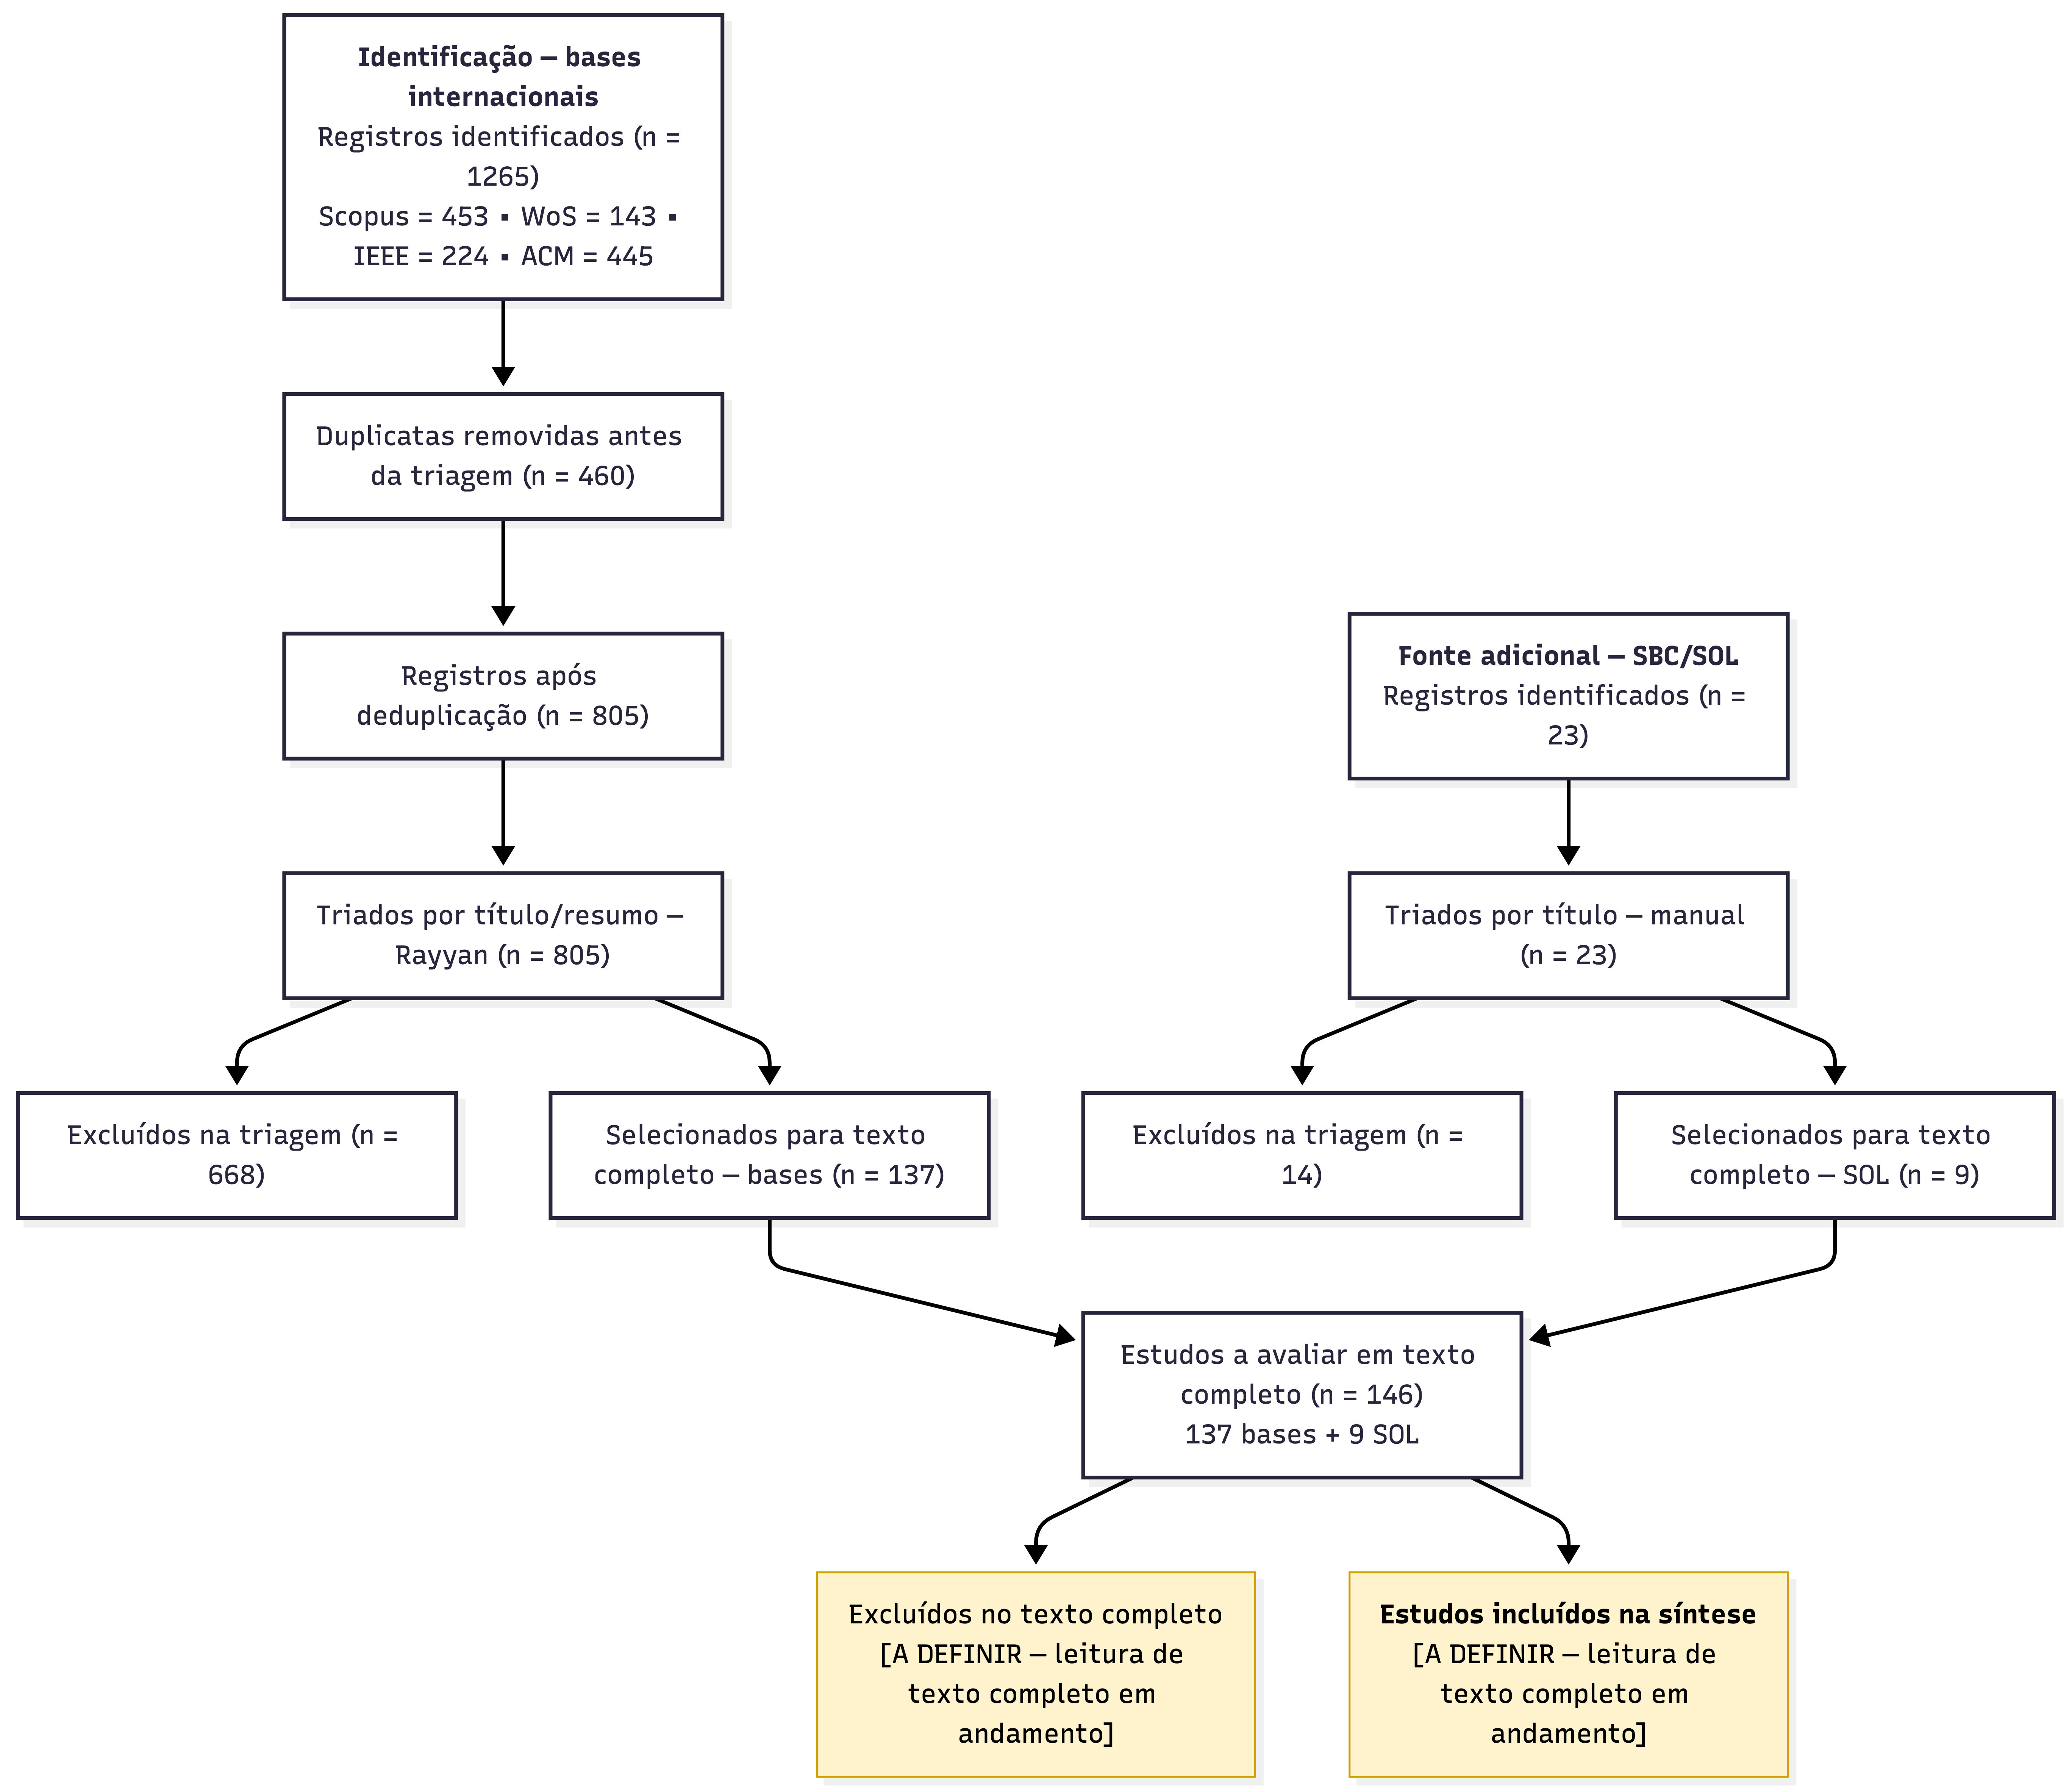
\includegraphics[width=0.6\textwidth]{imagens/fluxograma_execucao.png}
\caption{Fluxo de seleção dos estudos (PRISMA).}
\label{fig:prisma}
\end{figure*}

% Quantitativos de identificação, deduplicação e triagem atualizados para o protocolo
% consolidado (4 bases internacionais + SOL como fonte adicional). A inclusão final na
% síntese permanece pendente da leitura de texto completo (nó [A DEFINIR] na
% Figura~\ref{fig:prisma}); o snowballing está previsto sobre o corpus consolidado.

\noindent\textbf{[Em consolidação]} A caracterização do corpus e a síntese das questões de pesquisa (RQ1--RQ5), assim como a tabela de estudos incluídos, dependem da conclusão da leitura de texto completo dos 142 estudos selecionados (ver Seção~\ref{subsec:res_selecao}). A síntese da execução preliminar (7 estudos) foi preservada no código-fonte e será substituída pelo corpus consolidado; não é exibida aqui para não conflitar com o número de incluídos ainda [A DEFINIR].

% ===================================================================== %
% BLOCO 4.2-4.8 OCULTADO DA COMPILACAO (\iffalse ... \fi).               %
% Conteudo PRESERVADO para reescrita apos a leitura de texto completo    %
% dos 142 estudos. NAO APAGAR. Sintese da execucao preliminar (7         %
% estudos) que contradiz o numero de incluidos [A DEFINIR] do Sec. 4.1.  %
% As refs Colombo2025/Colombo2024/VonLuckeFrank2025/Kim2025/Mendes2025/  %
% PapadopoulosCharalabidis2020 caem das Referencias enquanto oculto      %
% (comportamento correto); voltam quando o bloco for recitado.           %
% ===================================================================== %
\iffalse
\subsection{Caracterização dos Estudos Incluídos}
\label{subsec:res_carac}

O corpus reúne trabalhos recentes — predominantemente posteriores a 2022 — concentrados em contextos europeus e asiáticos, com participação pontual de estudos sobre o contexto brasileiro. A Tabela~\ref{tab:corpus} sumariza os estudos incluídos quanto a foco, contexto e abordagem.

Registra-se uma decisão de escopo: três dos sete estudos recuperados --- \citet{Mendes2025}, \citet{Bojars2019} e \citet{PapadopoulosCharalabidis2020} --- empregam PLN clássico ou \textit{Linked Data}, e não IA Generativa. Por não satisfazerem plenamente o critério CI1, são aqui tratados como \textbf{contexto comparativo} e não compõem a base de evidências das questões sobre uso de LLMs (RQ3 em diante), restando \mbox{$n \approx 4$} estudos efetivamente generativos. % TODO: na execução final, reaplicar CI/CE e consolidar o corpus generativo (excluir formalmente ou redefinir o escopo e as RQs).

\begin{table*}[t]
\centering
\caption{Estudos primários incluídos na execução preliminar}
\label{tab:corpus}
\small
\begin{tabular}{|p{3.0cm}|p{2.3cm}|p{5.2cm}|}
\hline
\textbf{Estudo} & \textbf{Contexto} & \textbf{Foco / abordagem} \\
\hline
\citet{Colombo2025} & Itália & \textit{Pipeline} assistido por LLM para construção de \textit{knowledge graphs} da legislação \\
\hline
\citet{Colombo2024} & Itália & Sinergia entre grafos de conhecimento e LLMs para monitoramento e versionamento de legislação \\
\hline
\citet{VonLuckeFrank2025} & Parlamentos (geral) & Uso de ChatGPT em parlamentos; potencialidades e riscos (alucinação, imprecisão) \\
\hline
\citet{Kim2025} & Coreia do Sul & \textit{LegisFlow}: interface conversacional com consciência temporal, avaliada com usuários \\
\hline
\citet{Mendes2025} & Brasil & \textit{Topic Modeling} (PLN clássico) sobre Pedidos de Acesso à Informação \\
\hline
\citet{Bojars2019} & Letônia & \textit{LinkedSaeima}: dados parlamentares abertos conectados (\textit{Linked Data}) \\
\hline
\citet{PapadopoulosCharalabidis2020} & Estratégias nacionais de IA & PLN para mineração de \textit{insights} em documentos governamentais \\
\hline
\end{tabular}
\end{table*}

\subsection{RQ1 --- Aplicações de IA Generativa em Governo Aberto}
\label{subsec:res_rq1}

As aplicações de IA Generativa identificadas concentram-se em dois eixos. O primeiro é a \textbf{estruturação de dados legislativos}: \citet{Colombo2025} e \citet{Colombo2024} empregam LLMs para extrair entidades jurídicas de textos não estruturados e organizá-las em grafos de conhecimento, viabilizando inclusive o monitoramento da evolução das leis. O segundo é o \textbf{acesso conversacional}: \citet{Kim2025} implementam um \textit{chatbot} para consultas em linguagem natural sobre legislação, e \citet{VonLuckeFrank2025} discutem o uso de ChatGPT para síntese e apoio em contextos parlamentares. Os demais estudos do corpus recorrem a PLN clássico ou a \textit{Linked Data} \citep{Mendes2025,Bojars2019,PapadopoulosCharalabidis2020}, e não à IA Generativa — o que delimita o subconjunto efetivamente generativo da literatura recuperada.

\subsection{RQ2 --- Tipos de Dados Governamentais}
\label{subsec:res_rq2}

Os dados analisados abrangem textos de legislação e sua evolução temporal \citep{Colombo2025,Colombo2024}, atividade e documentos parlamentares \citep{Kim2025,Bojars2019}, Pedidos de Acesso à Informação \citep{Mendes2025} e documentos de estratégias governamentais de IA \citep{PapadopoulosCharalabidis2020}. Predominam dados textuais não estruturados, o que motiva o uso de técnicas de processamento de linguagem natural — generativas ou clássicas — para sua estruturação e consulta.

\subsection{RQ3 --- LLMs Utilizados}
\label{subsec:res_rq3}

Entre os estudos generativos, \citet{VonLuckeFrank2025} examinam explicitamente o ChatGPT, enquanto \citet{Colombo2025,Colombo2024} reportam o uso de LLMs como assistentes na construção de grafos de conhecimento sem, em geral, fixar um modelo único, e \citet{Kim2025} apoiam o \textit{LegisFlow} em modelos de linguagem. Observa-se que parte relevante do corpus ainda não adota LLMs, recorrendo a abordagens clássicas — uma lacuna discutida adiante.
% TODO (após extensão): consolidar modelos, porte e licença (aberto/proprietário)
% em tabela, conforme o formulário de extração (Tabela de extração do Método).

\subsection{RQ4 --- Benefícios Reportados}
\label{subsec:res_rq4}

Os benefícios relatados incluem a transformação de dados legislativos complexos em estruturas de conhecimento compreensíveis \citep{Colombo2025}, o rastreamento da evolução normativa ao longo do tempo \citep{Colombo2024}, a redução da barreira de entrada ao acesso legislativo por meio de interação em linguagem natural \citep{Kim2025} e o ganho de rapidez na síntese de informações \citep{VonLuckeFrank2025}. Esses benefícios, contudo, são em larga medida \textbf{autodeclarados} pelos estudos primários e apoiados em um corpus reduzido (\mbox{$n \approx 4$} estudos efetivamente generativos), o que recomenda interpretá-los como indícios preliminares de potencial, e não como evidência consolidada.

\subsection{RQ5 --- Desafios e Limitações}
\label{subsec:res_rq5}

O desafio mais saliente é a \textbf{confiabilidade} das respostas geradas: \citet{VonLuckeFrank2025} alertam para riscos de alucinação e imprecisão factual, sem que a literatura recuperada apresente estratégias sistemáticas de validação. Soma-se a isso a escassez de foco em \textbf{acessibilidade para o cidadão não especialista}, já que vários trabalhos priorizam a estruturação técnica, e a sub-representação do \textbf{contexto brasileiro e da língua portuguesa}. Por fim, a integração de múltiplas modalidades de interação (por exemplo, \textit{dashboard} e \textit{chatbot}) é raramente explorada de forma conjunta.

\subsection{Lacunas e Agenda de Pesquisa}
\label{subsec:res_lacunas}

A síntese evidencia um campo em formação. As principais lacunas identificadas são: (i) o foco predominante na estruturação técnica, em detrimento da acessibilidade ao cidadão; (ii) a ausência de protocolos sistemáticos para avaliação da confiabilidade e da rastreabilidade das respostas geradas; (iii) a baixa cobertura de contextos não europeus/asiáticos, em especial o brasileiro e em língua portuguesa; e (iv) a rara integração de modalidades de interação. Dado o tamanho reduzido do corpus desta execução preliminar, essas lacunas devem ser lidas como \textbf{hipóteses de pesquisa} a confirmar com o corpus ampliado, e não como conclusões consolidadas; ainda assim, orientam uma agenda de pesquisa em Sistemas de Informação na interseção entre IA Generativa, dados abertos e transparência pública.

% TODO (após extensão): rever as lacunas à luz do corpus ampliado e quantificar,
% quando possível, a distribuição dos estudos por RQ.
\fi
% ===================================================================== %
% FIM DO BLOCO 4.2-4.8 OCULTADO (\iffalse ... \fi).                      %
% ===================================================================== %

%
%  ORIGEM: migração do Mapeamento Sistemático já conduzido na dissertação
%  (capitulos/estado_arte.tex). Conversões aplicadas:
%   \quadro -> table | \citeonline -> \citet | \cite -> \citep | \fonte removido.
%
%  >>> EXECUÇÃO PRELIMINAR <<<  Os números e o corpus (7 estudos) referem-se à
%  execução INICIAL do mapeamento (5 bases, janela 2014–2026, busca em maio/2026,
%  questões Q1–Q4 da dissertação). A consolidação para o protocolo desta RSL
%  (4 bases internacionais + snowballing; RQ1–RQ5) está em andamento; os
%  quantitativos serão ATUALIZADOS após a extensão. Manter as notas % TODO.
% =====================================================================

\section{Resultados}
\label{sec:resultados}

Esta seção reporta os resultados da execução inicial da revisão, que constitui a base a ser ampliada pelo \textit{snowballing} e pela consolidação do protocolo descrito na Seção~\ref{sec:metodo}. Os achados são apresentados na ordem do processo: seleção dos estudos (PRISMA), caracterização do corpus e síntese organizada pelas questões de pesquisa.

\subsection{Seleção dos Estudos}
\label{subsec:res_selecao}

A busca automática nas quatro bases internacionais recuperou 1265 registros, assim distribuídos: Scopus (453), ACM Digital Library (445), IEEE Xplore (224) e Web of Science (143). Como fonte adicional, a busca na Biblioteca Digital da SBC/SOL recuperou 23 registros, tratados em fluxo separado por essa base não oferecer exportação padronizada (BibTeX/RIS). A deduplicação das quatro bases internacionais, conduzida no Zotero, removeu 460 registros, resultando em 805 registros únicos; os 23 registros da SOL foram deduplicados manualmente. Na triagem por título e resumo, operacionalizada no Rayyan, os 805 registros das bases internacionais levaram a 668 exclusões e a 137 estudos encaminhados à leitura de texto completo; na SOL, dos 23 registros, 18 foram excluídos e 5 encaminhados ao texto completo (2 inclusões firmes e 3 a confirmar). A etapa de leitura de texto completo abrange, portanto, 142 estudos (137 das bases internacionais e 5 da SOL). O número de estudos incluídos na síntese encontra-se [A DEFINIR --- leitura de texto completo em andamento]. A Figura~\ref{fig:prisma} sintetiza o fluxo de identificação, deduplicação, triagem e elegibilidade.

\begin{figure*}[t]
\centering
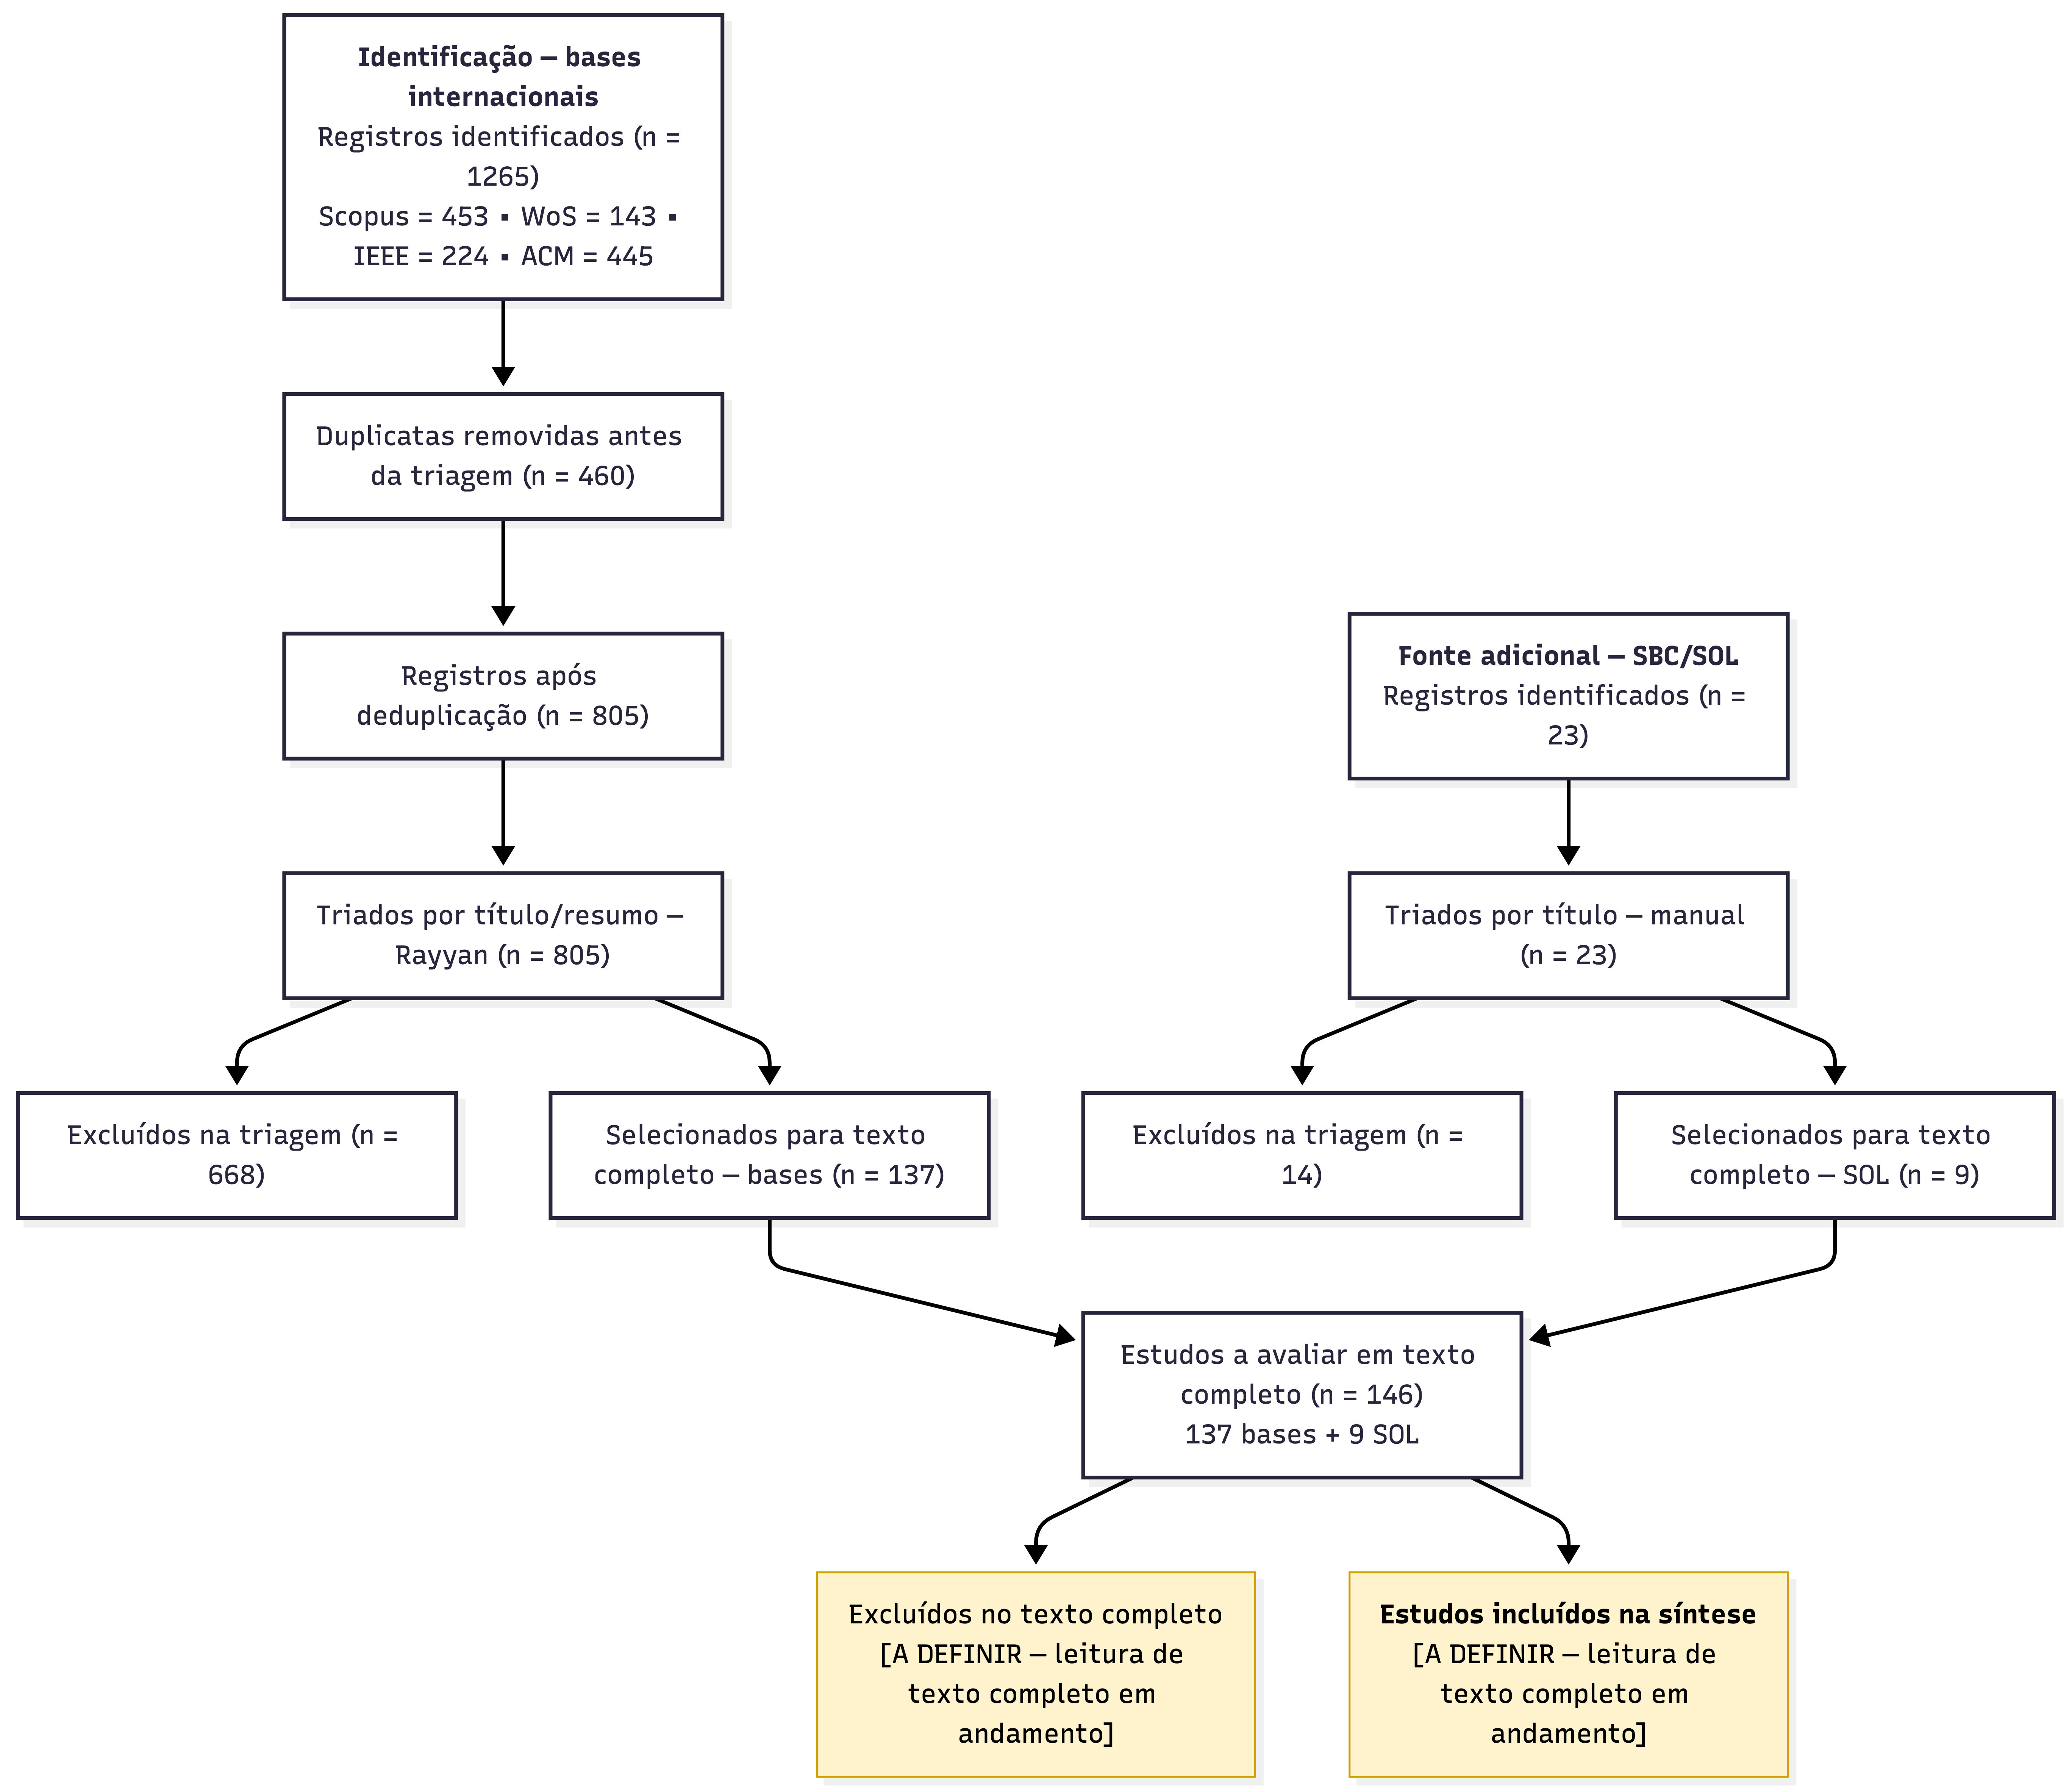
\includegraphics[width=0.6\textwidth]{imagens/fluxograma_execucao.png}
\caption{Fluxo de seleção dos estudos (PRISMA).}
\label{fig:prisma}
\end{figure*}

% Quantitativos de identificação, deduplicação e triagem atualizados para o protocolo
% consolidado (4 bases internacionais + SOL como fonte adicional). A inclusão final na
% síntese permanece pendente da leitura de texto completo (nó [A DEFINIR] na
% Figura~\ref{fig:prisma}); o snowballing está previsto sobre o corpus consolidado.

\noindent\textbf{[Em consolidação]} A caracterização do corpus e a síntese das questões de pesquisa (RQ1--RQ5), assim como a tabela de estudos incluídos, dependem da conclusão da leitura de texto completo dos 142 estudos selecionados (ver Seção~\ref{subsec:res_selecao}). A síntese da execução preliminar (7 estudos) foi preservada no código-fonte e será substituída pelo corpus consolidado; não é exibida aqui para não conflitar com o número de incluídos ainda [A DEFINIR].

% ===================================================================== %
% BLOCO 4.2-4.8 OCULTADO DA COMPILACAO (\iffalse ... \fi).               %
% Conteudo PRESERVADO para reescrita apos a leitura de texto completo    %
% dos 142 estudos. NAO APAGAR. Sintese da execucao preliminar (7         %
% estudos) que contradiz o numero de incluidos [A DEFINIR] do Sec. 4.1.  %
% As refs Colombo2025/Colombo2024/VonLuckeFrank2025/Kim2025/Mendes2025/  %
% PapadopoulosCharalabidis2020 caem das Referencias enquanto oculto      %
% (comportamento correto); voltam quando o bloco for recitado.           %
% ===================================================================== %
\iffalse
\subsection{Caracterização dos Estudos Incluídos}
\label{subsec:res_carac}

O corpus reúne trabalhos recentes — predominantemente posteriores a 2022 — concentrados em contextos europeus e asiáticos, com participação pontual de estudos sobre o contexto brasileiro. A Tabela~\ref{tab:corpus} sumariza os estudos incluídos quanto a foco, contexto e abordagem.

Registra-se uma decisão de escopo: três dos sete estudos recuperados --- \citet{Mendes2025}, \citet{Bojars2019} e \citet{PapadopoulosCharalabidis2020} --- empregam PLN clássico ou \textit{Linked Data}, e não IA Generativa. Por não satisfazerem plenamente o critério CI1, são aqui tratados como \textbf{contexto comparativo} e não compõem a base de evidências das questões sobre uso de LLMs (RQ3 em diante), restando \mbox{$n \approx 4$} estudos efetivamente generativos. % TODO: na execução final, reaplicar CI/CE e consolidar o corpus generativo (excluir formalmente ou redefinir o escopo e as RQs).

\begin{table*}[t]
\centering
\caption{Estudos primários incluídos na execução preliminar}
\label{tab:corpus}
\small
\begin{tabular}{|p{3.0cm}|p{2.3cm}|p{5.2cm}|}
\hline
\textbf{Estudo} & \textbf{Contexto} & \textbf{Foco / abordagem} \\
\hline
\citet{Colombo2025} & Itália & \textit{Pipeline} assistido por LLM para construção de \textit{knowledge graphs} da legislação \\
\hline
\citet{Colombo2024} & Itália & Sinergia entre grafos de conhecimento e LLMs para monitoramento e versionamento de legislação \\
\hline
\citet{VonLuckeFrank2025} & Parlamentos (geral) & Uso de ChatGPT em parlamentos; potencialidades e riscos (alucinação, imprecisão) \\
\hline
\citet{Kim2025} & Coreia do Sul & \textit{LegisFlow}: interface conversacional com consciência temporal, avaliada com usuários \\
\hline
\citet{Mendes2025} & Brasil & \textit{Topic Modeling} (PLN clássico) sobre Pedidos de Acesso à Informação \\
\hline
\citet{Bojars2019} & Letônia & \textit{LinkedSaeima}: dados parlamentares abertos conectados (\textit{Linked Data}) \\
\hline
\citet{PapadopoulosCharalabidis2020} & Estratégias nacionais de IA & PLN para mineração de \textit{insights} em documentos governamentais \\
\hline
\end{tabular}
\end{table*}

\subsection{RQ1 --- Aplicações de IA Generativa em Governo Aberto}
\label{subsec:res_rq1}

As aplicações de IA Generativa identificadas concentram-se em dois eixos. O primeiro é a \textbf{estruturação de dados legislativos}: \citet{Colombo2025} e \citet{Colombo2024} empregam LLMs para extrair entidades jurídicas de textos não estruturados e organizá-las em grafos de conhecimento, viabilizando inclusive o monitoramento da evolução das leis. O segundo é o \textbf{acesso conversacional}: \citet{Kim2025} implementam um \textit{chatbot} para consultas em linguagem natural sobre legislação, e \citet{VonLuckeFrank2025} discutem o uso de ChatGPT para síntese e apoio em contextos parlamentares. Os demais estudos do corpus recorrem a PLN clássico ou a \textit{Linked Data} \citep{Mendes2025,Bojars2019,PapadopoulosCharalabidis2020}, e não à IA Generativa — o que delimita o subconjunto efetivamente generativo da literatura recuperada.

\subsection{RQ2 --- Tipos de Dados Governamentais}
\label{subsec:res_rq2}

Os dados analisados abrangem textos de legislação e sua evolução temporal \citep{Colombo2025,Colombo2024}, atividade e documentos parlamentares \citep{Kim2025,Bojars2019}, Pedidos de Acesso à Informação \citep{Mendes2025} e documentos de estratégias governamentais de IA \citep{PapadopoulosCharalabidis2020}. Predominam dados textuais não estruturados, o que motiva o uso de técnicas de processamento de linguagem natural — generativas ou clássicas — para sua estruturação e consulta.

\subsection{RQ3 --- LLMs Utilizados}
\label{subsec:res_rq3}

Entre os estudos generativos, \citet{VonLuckeFrank2025} examinam explicitamente o ChatGPT, enquanto \citet{Colombo2025,Colombo2024} reportam o uso de LLMs como assistentes na construção de grafos de conhecimento sem, em geral, fixar um modelo único, e \citet{Kim2025} apoiam o \textit{LegisFlow} em modelos de linguagem. Observa-se que parte relevante do corpus ainda não adota LLMs, recorrendo a abordagens clássicas — uma lacuna discutida adiante.
% TODO (após extensão): consolidar modelos, porte e licença (aberto/proprietário)
% em tabela, conforme o formulário de extração (Tabela de extração do Método).

\subsection{RQ4 --- Benefícios Reportados}
\label{subsec:res_rq4}

Os benefícios relatados incluem a transformação de dados legislativos complexos em estruturas de conhecimento compreensíveis \citep{Colombo2025}, o rastreamento da evolução normativa ao longo do tempo \citep{Colombo2024}, a redução da barreira de entrada ao acesso legislativo por meio de interação em linguagem natural \citep{Kim2025} e o ganho de rapidez na síntese de informações \citep{VonLuckeFrank2025}. Esses benefícios, contudo, são em larga medida \textbf{autodeclarados} pelos estudos primários e apoiados em um corpus reduzido (\mbox{$n \approx 4$} estudos efetivamente generativos), o que recomenda interpretá-los como indícios preliminares de potencial, e não como evidência consolidada.

\subsection{RQ5 --- Desafios e Limitações}
\label{subsec:res_rq5}

O desafio mais saliente é a \textbf{confiabilidade} das respostas geradas: \citet{VonLuckeFrank2025} alertam para riscos de alucinação e imprecisão factual, sem que a literatura recuperada apresente estratégias sistemáticas de validação. Soma-se a isso a escassez de foco em \textbf{acessibilidade para o cidadão não especialista}, já que vários trabalhos priorizam a estruturação técnica, e a sub-representação do \textbf{contexto brasileiro e da língua portuguesa}. Por fim, a integração de múltiplas modalidades de interação (por exemplo, \textit{dashboard} e \textit{chatbot}) é raramente explorada de forma conjunta.

\subsection{Lacunas e Agenda de Pesquisa}
\label{subsec:res_lacunas}

A síntese evidencia um campo em formação. As principais lacunas identificadas são: (i) o foco predominante na estruturação técnica, em detrimento da acessibilidade ao cidadão; (ii) a ausência de protocolos sistemáticos para avaliação da confiabilidade e da rastreabilidade das respostas geradas; (iii) a baixa cobertura de contextos não europeus/asiáticos, em especial o brasileiro e em língua portuguesa; e (iv) a rara integração de modalidades de interação. Dado o tamanho reduzido do corpus desta execução preliminar, essas lacunas devem ser lidas como \textbf{hipóteses de pesquisa} a confirmar com o corpus ampliado, e não como conclusões consolidadas; ainda assim, orientam uma agenda de pesquisa em Sistemas de Informação na interseção entre IA Generativa, dados abertos e transparência pública.

% TODO (após extensão): rever as lacunas à luz do corpus ampliado e quantificar,
% quando possível, a distribuição dos estudos por RQ.
\fi
% ===================================================================== %
% FIM DO BLOCO 4.2-4.8 OCULTADO (\iffalse ... \fi).                      %
% ===================================================================== %

%
%  ORIGEM: migração do Mapeamento Sistemático já conduzido na dissertação
%  (capitulos/estado_arte.tex). Conversões aplicadas:
%   \quadro -> table | \citeonline -> \citet | \cite -> \citep | \fonte removido.
%
%  >>> EXECUÇÃO PRELIMINAR <<<  Os números e o corpus (7 estudos) referem-se à
%  execução INICIAL do mapeamento (5 bases, janela 2014–2026, busca em maio/2026,
%  questões Q1–Q4 da dissertação). A consolidação para o protocolo desta RSL
%  (4 bases internacionais + snowballing; RQ1–RQ5) está em andamento; os
%  quantitativos serão ATUALIZADOS após a extensão. Manter as notas % TODO.
% =====================================================================

\section{Resultados}
\label{sec:resultados}

Esta seção reporta os resultados da execução inicial da revisão, que constitui a base a ser ampliada pelo \textit{snowballing} e pela consolidação do protocolo descrito na Seção~\ref{sec:metodo}. Os achados são apresentados na ordem do processo: seleção dos estudos (PRISMA), caracterização do corpus e síntese organizada pelas questões de pesquisa.

\subsection{Seleção dos Estudos}
\label{subsec:res_selecao}

A busca automática nas quatro bases internacionais recuperou 1265 registros, assim distribuídos: Scopus (453), ACM Digital Library (445), IEEE Xplore (224) e Web of Science (143). Como fonte adicional, a busca na Biblioteca Digital da SBC/SOL recuperou 23 registros, tratados em fluxo separado por essa base não oferecer exportação padronizada (BibTeX/RIS). A deduplicação das quatro bases internacionais, conduzida no Zotero, removeu 460 registros, resultando em 805 registros únicos; os 23 registros da SOL foram deduplicados manualmente. Na triagem por título e resumo, operacionalizada no Rayyan, os 805 registros das bases internacionais levaram a 668 exclusões e a 137 estudos encaminhados à leitura de texto completo; na SOL, dos 23 registros, 18 foram excluídos e 5 encaminhados ao texto completo (2 inclusões firmes e 3 a confirmar). A etapa de leitura de texto completo abrange, portanto, 142 estudos (137 das bases internacionais e 5 da SOL). O número de estudos incluídos na síntese encontra-se [A DEFINIR --- leitura de texto completo em andamento]. A Figura~\ref{fig:prisma} sintetiza o fluxo de identificação, deduplicação, triagem e elegibilidade.

\begin{figure*}[t]
\centering
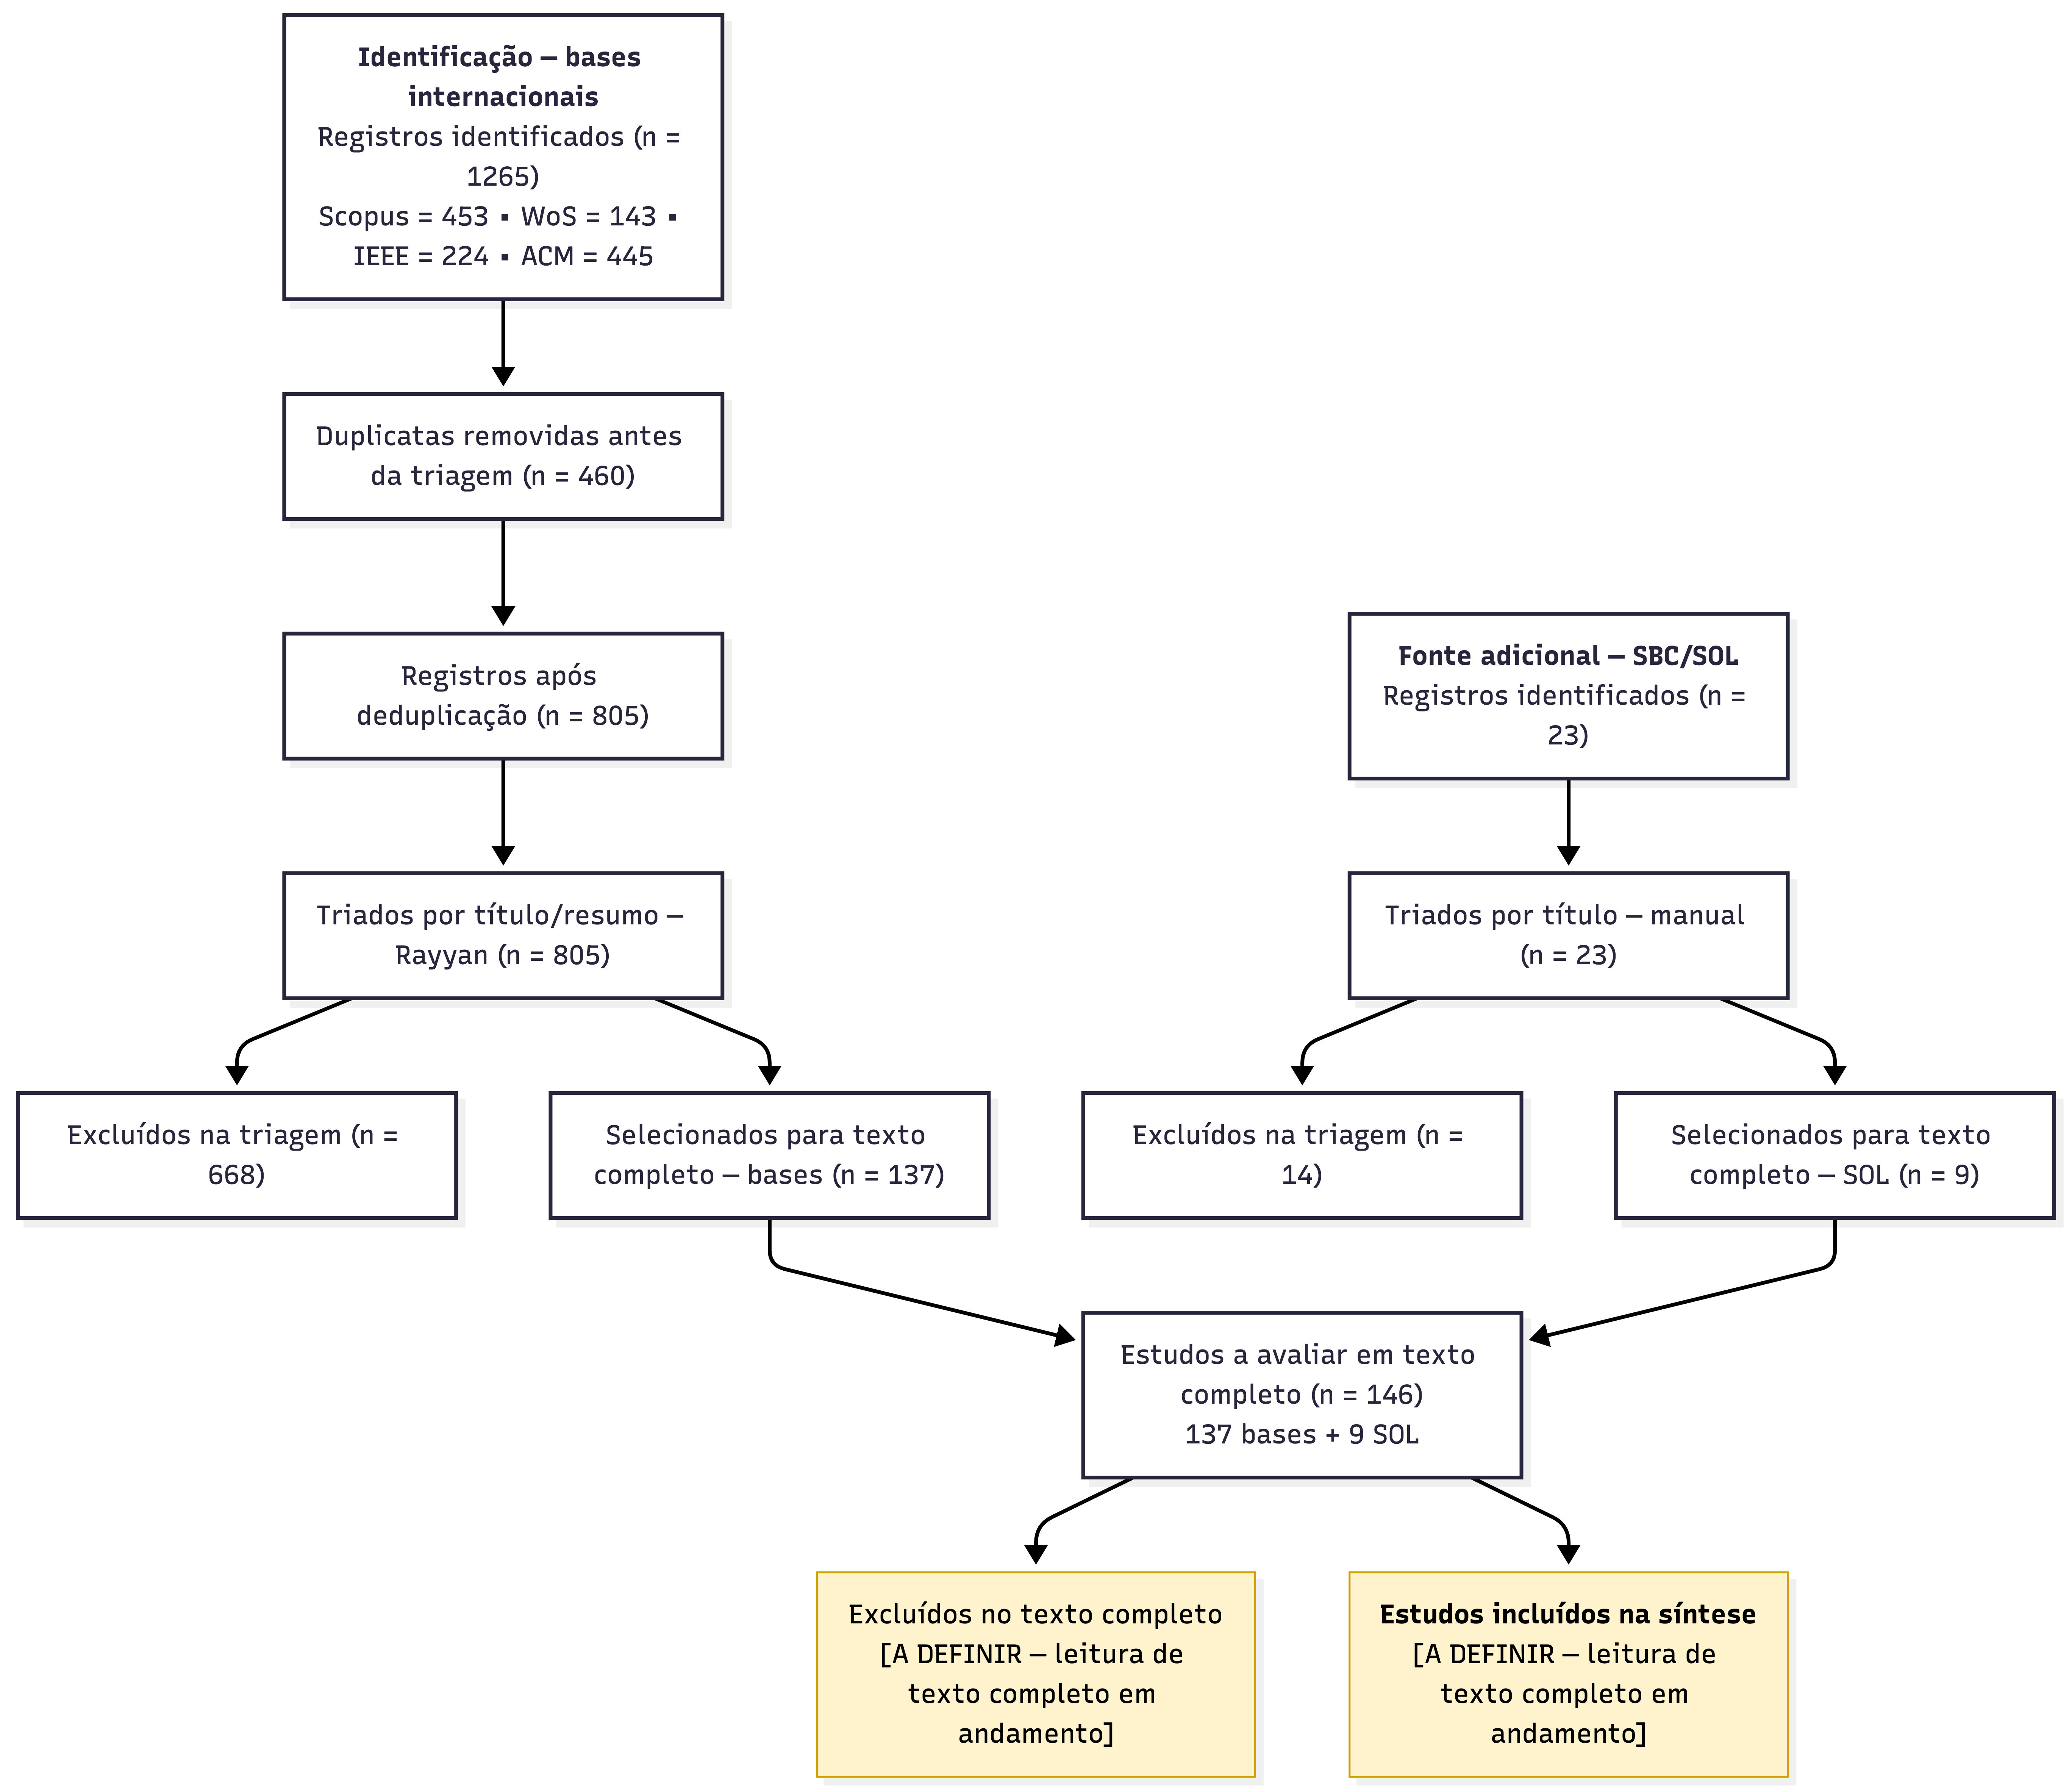
\includegraphics[width=0.6\textwidth]{imagens/fluxograma_execucao.png}
\caption{Fluxo de seleção dos estudos (PRISMA).}
\label{fig:prisma}
\end{figure*}

% Quantitativos de identificação, deduplicação e triagem atualizados para o protocolo
% consolidado (4 bases internacionais + SOL como fonte adicional). A inclusão final na
% síntese permanece pendente da leitura de texto completo (nó [A DEFINIR] na
% Figura~\ref{fig:prisma}); o snowballing está previsto sobre o corpus consolidado.

\noindent\textbf{[Em consolidação]} A caracterização do corpus e a síntese das questões de pesquisa (RQ1--RQ5), assim como a tabela de estudos incluídos, dependem da conclusão da leitura de texto completo dos 142 estudos selecionados (ver Seção~\ref{subsec:res_selecao}). A síntese da execução preliminar (7 estudos) foi preservada no código-fonte e será substituída pelo corpus consolidado; não é exibida aqui para não conflitar com o número de incluídos ainda [A DEFINIR].

% ===================================================================== %
% BLOCO 4.2-4.8 OCULTADO DA COMPILACAO (\iffalse ... \fi).               %
% Conteudo PRESERVADO para reescrita apos a leitura de texto completo    %
% dos 142 estudos. NAO APAGAR. Sintese da execucao preliminar (7         %
% estudos) que contradiz o numero de incluidos [A DEFINIR] do Sec. 4.1.  %
% As refs Colombo2025/Colombo2024/VonLuckeFrank2025/Kim2025/Mendes2025/  %
% PapadopoulosCharalabidis2020 caem das Referencias enquanto oculto      %
% (comportamento correto); voltam quando o bloco for recitado.           %
% ===================================================================== %
\iffalse
\subsection{Caracterização dos Estudos Incluídos}
\label{subsec:res_carac}

O corpus reúne trabalhos recentes — predominantemente posteriores a 2022 — concentrados em contextos europeus e asiáticos, com participação pontual de estudos sobre o contexto brasileiro. A Tabela~\ref{tab:corpus} sumariza os estudos incluídos quanto a foco, contexto e abordagem.

Registra-se uma decisão de escopo: três dos sete estudos recuperados --- \citet{Mendes2025}, \citet{Bojars2019} e \citet{PapadopoulosCharalabidis2020} --- empregam PLN clássico ou \textit{Linked Data}, e não IA Generativa. Por não satisfazerem plenamente o critério CI1, são aqui tratados como \textbf{contexto comparativo} e não compõem a base de evidências das questões sobre uso de LLMs (RQ3 em diante), restando \mbox{$n \approx 4$} estudos efetivamente generativos. % TODO: na execução final, reaplicar CI/CE e consolidar o corpus generativo (excluir formalmente ou redefinir o escopo e as RQs).

\begin{table*}[t]
\centering
\caption{Estudos primários incluídos na execução preliminar}
\label{tab:corpus}
\small
\begin{tabular}{|p{3.0cm}|p{2.3cm}|p{5.2cm}|}
\hline
\textbf{Estudo} & \textbf{Contexto} & \textbf{Foco / abordagem} \\
\hline
\citet{Colombo2025} & Itália & \textit{Pipeline} assistido por LLM para construção de \textit{knowledge graphs} da legislação \\
\hline
\citet{Colombo2024} & Itália & Sinergia entre grafos de conhecimento e LLMs para monitoramento e versionamento de legislação \\
\hline
\citet{VonLuckeFrank2025} & Parlamentos (geral) & Uso de ChatGPT em parlamentos; potencialidades e riscos (alucinação, imprecisão) \\
\hline
\citet{Kim2025} & Coreia do Sul & \textit{LegisFlow}: interface conversacional com consciência temporal, avaliada com usuários \\
\hline
\citet{Mendes2025} & Brasil & \textit{Topic Modeling} (PLN clássico) sobre Pedidos de Acesso à Informação \\
\hline
\citet{Bojars2019} & Letônia & \textit{LinkedSaeima}: dados parlamentares abertos conectados (\textit{Linked Data}) \\
\hline
\citet{PapadopoulosCharalabidis2020} & Estratégias nacionais de IA & PLN para mineração de \textit{insights} em documentos governamentais \\
\hline
\end{tabular}
\end{table*}

\subsection{RQ1 --- Aplicações de IA Generativa em Governo Aberto}
\label{subsec:res_rq1}

As aplicações de IA Generativa identificadas concentram-se em dois eixos. O primeiro é a \textbf{estruturação de dados legislativos}: \citet{Colombo2025} e \citet{Colombo2024} empregam LLMs para extrair entidades jurídicas de textos não estruturados e organizá-las em grafos de conhecimento, viabilizando inclusive o monitoramento da evolução das leis. O segundo é o \textbf{acesso conversacional}: \citet{Kim2025} implementam um \textit{chatbot} para consultas em linguagem natural sobre legislação, e \citet{VonLuckeFrank2025} discutem o uso de ChatGPT para síntese e apoio em contextos parlamentares. Os demais estudos do corpus recorrem a PLN clássico ou a \textit{Linked Data} \citep{Mendes2025,Bojars2019,PapadopoulosCharalabidis2020}, e não à IA Generativa — o que delimita o subconjunto efetivamente generativo da literatura recuperada.

\subsection{RQ2 --- Tipos de Dados Governamentais}
\label{subsec:res_rq2}

Os dados analisados abrangem textos de legislação e sua evolução temporal \citep{Colombo2025,Colombo2024}, atividade e documentos parlamentares \citep{Kim2025,Bojars2019}, Pedidos de Acesso à Informação \citep{Mendes2025} e documentos de estratégias governamentais de IA \citep{PapadopoulosCharalabidis2020}. Predominam dados textuais não estruturados, o que motiva o uso de técnicas de processamento de linguagem natural — generativas ou clássicas — para sua estruturação e consulta.

\subsection{RQ3 --- LLMs Utilizados}
\label{subsec:res_rq3}

Entre os estudos generativos, \citet{VonLuckeFrank2025} examinam explicitamente o ChatGPT, enquanto \citet{Colombo2025,Colombo2024} reportam o uso de LLMs como assistentes na construção de grafos de conhecimento sem, em geral, fixar um modelo único, e \citet{Kim2025} apoiam o \textit{LegisFlow} em modelos de linguagem. Observa-se que parte relevante do corpus ainda não adota LLMs, recorrendo a abordagens clássicas — uma lacuna discutida adiante.
% TODO (após extensão): consolidar modelos, porte e licença (aberto/proprietário)
% em tabela, conforme o formulário de extração (Tabela de extração do Método).

\subsection{RQ4 --- Benefícios Reportados}
\label{subsec:res_rq4}

Os benefícios relatados incluem a transformação de dados legislativos complexos em estruturas de conhecimento compreensíveis \citep{Colombo2025}, o rastreamento da evolução normativa ao longo do tempo \citep{Colombo2024}, a redução da barreira de entrada ao acesso legislativo por meio de interação em linguagem natural \citep{Kim2025} e o ganho de rapidez na síntese de informações \citep{VonLuckeFrank2025}. Esses benefícios, contudo, são em larga medida \textbf{autodeclarados} pelos estudos primários e apoiados em um corpus reduzido (\mbox{$n \approx 4$} estudos efetivamente generativos), o que recomenda interpretá-los como indícios preliminares de potencial, e não como evidência consolidada.

\subsection{RQ5 --- Desafios e Limitações}
\label{subsec:res_rq5}

O desafio mais saliente é a \textbf{confiabilidade} das respostas geradas: \citet{VonLuckeFrank2025} alertam para riscos de alucinação e imprecisão factual, sem que a literatura recuperada apresente estratégias sistemáticas de validação. Soma-se a isso a escassez de foco em \textbf{acessibilidade para o cidadão não especialista}, já que vários trabalhos priorizam a estruturação técnica, e a sub-representação do \textbf{contexto brasileiro e da língua portuguesa}. Por fim, a integração de múltiplas modalidades de interação (por exemplo, \textit{dashboard} e \textit{chatbot}) é raramente explorada de forma conjunta.

\subsection{Lacunas e Agenda de Pesquisa}
\label{subsec:res_lacunas}

A síntese evidencia um campo em formação. As principais lacunas identificadas são: (i) o foco predominante na estruturação técnica, em detrimento da acessibilidade ao cidadão; (ii) a ausência de protocolos sistemáticos para avaliação da confiabilidade e da rastreabilidade das respostas geradas; (iii) a baixa cobertura de contextos não europeus/asiáticos, em especial o brasileiro e em língua portuguesa; e (iv) a rara integração de modalidades de interação. Dado o tamanho reduzido do corpus desta execução preliminar, essas lacunas devem ser lidas como \textbf{hipóteses de pesquisa} a confirmar com o corpus ampliado, e não como conclusões consolidadas; ainda assim, orientam uma agenda de pesquisa em Sistemas de Informação na interseção entre IA Generativa, dados abertos e transparência pública.

% TODO (após extensão): rever as lacunas à luz do corpus ampliado e quantificar,
% quando possível, a distribuição dos estudos por RQ.
\fi
% ===================================================================== %
% FIM DO BLOCO 4.2-4.8 OCULTADO (\iffalse ... \fi).                      %
% ===================================================================== %


% =====================================================================
\section{Discussão}
\label{sec:discussao}
% =====================================================================
% TODO: síntese transversal, implicações para pesquisa e prática em Sistemas
% de Informação, e agenda de pesquisa.
\textbf{[TODO (depende da revisão conduzida)]}

% =====================================================================
\section{Ameaças à Validade}
\label{sec:ameacas}
% =====================================================================
% Estrutura reaproveitável de capitulos/consideracoes.tex (arquivado).
\begin{description}
  \item[Validade de construto] Adequação das RQs e da \emph{string} de busca ao
        fenômeno; risco de os termos não capturarem trabalhos relevantes.
        \emph{Mitigação:} string iterada por especialista e \emph{snowballing}.
        % [TODO-transparência] Nota para mim mesma (NÃO é o texto final): declarar
        % que a transparência pública entra como HORIZONTE/MOTIVAÇÃO do estudo, e
        % não necessariamente como desfecho medido. Após a busca reexecutada,
        % verificar se algum estudo do corpus final mede transparência como
        % DESFECHO (compreensão cidadã, accountability, uso efetivo): se SIM,
        % ancorar o título na evidência; se NÃO, declarar explicitamente aqui como
        % limitação de validade de construto. Fechar este parágrafo com os dados.
  \item[Validade interna] Vieses de seleção e extração, acentuados pelo fato de
        a revisão ter sido conduzida por uma única revisora, sem medida de
        concordância interavaliadores. \emph{Mitigação:} protocolo definido
        \emph{a priori}, critérios de inclusão/exclusão explícitos, e decisões de
        triagem e extração registradas de forma rastreável no Rayyan, permitindo
        auditoria; não se reivindica concordância entre revisores.
  \item[Validade externa] Generalização limitada pelo escopo de bases e idioma.
        \emph{Mitigação:} múltiplas bases e registro de limitações.
  \item[Validade de conclusão] Rastreabilidade entre dados extraídos e
        conclusões. \emph{Mitigação:} planilha de extração disponível (ver
        declaração de disponibilidade de dados).
\end{description}

% =====================================================================
\section{Conclusão}
\label{sec:conclusao}
% =====================================================================
% TODO: retomar objetivo, achados por RQ, contribuições para SI e trabalhos
% futuros.
\textbf{[TODO (depende da revisão conduzida)]}

% =====================================================================
%  DECLARAÇÕES OBRIGATÓRIAS iSys (bloco da classe)
% =====================================================================
\begin{declarations}

\begin{acknowledgements}
% OBRIGATÓRIA para publicação (se aceito). TODO: revisar/ajustar.
Os autores agradecem ao Programa de Pós-Graduação em Ciência da Computação da
Universidade Federal de Sergipe pelo apoio à pesquisa. % TODO: confirmar/ajustar.
\end{acknowledgements}

\begin{contributions}
% OBRIGATÓRIA (CRediT: https://credit.niso.org/). TODO: ajustar papéis.
A. B. C. Oliveira: conceituação, metodologia, condução da revisão (busca,
triagem e extração), redação do manuscrito original. G. J. F. da Silva:
supervisão, conceituação e revisão crítica do manuscrito. Todos os autores
leram e aprovaram a versão final.
\end{contributions}

\begin{interests}
% OBRIGATÓRIA.
Os autores declaram não haver conflitos de interesse.
\end{interests}

\begin{materials}
% OBRIGATÓRIA. Apontar repositório (GitHub/Zenodo) com protocolo, strings
% exatas por base, lista de estudos e planilha de extração.
% TODO: inserir DOI/URL do repositório.
O protocolo, as \textit{strings} de busca por base, a lista de estudos
incluídos e a planilha de extração estão disponíveis em repositório público:
\url{https://github.com/TODO}. % TODO: inserir URL/DOI (GitHub/Zenodo).
\end{materials}

\begin{funding}
% OBRIGATÓRIA para publicação (se aceito). TODO: confirmar.
Esta pesquisa não recebeu financiamento específico de agências de fomento dos
setores público, comercial ou sem fins lucrativos. % TODO: confirmar ou citar agência/processo.
\end{funding}

\begin{furtherinformation}
% DESEJÁVEL. Ética + uso de IA generativa.
Esta pesquisa utiliza exclusivamente dados públicos e literatura científica
publicada; não envolve participantes humanos, não coleta dados pessoais e não
manipula dados sensíveis, dispensando aprovação por comitê de ética.
% TODO: declarar, se aplicável, o uso de ferramentas de IA generativa na
% elaboração do artigo.
\end{furtherinformation}

\end{declarations}

% =====================================================================
%  REFERÊNCIAS — incluir DOI quando disponível (requisito do periódico).
%  Estilo: apalike-sol. Citações com \cite/\citep/\citet (natbib).
%  ATENÇÃO: referencias.bib vem do estilo ABNT (abntex2-alf); ao migrar
%  citações de estado_arte.tex, converter \citeonline -> \citet e revisar
%  as entradas .bib (DOI, formato apalike).
% =====================================================================
\bibliographystyle{apalike-sol}
\bibliography{referencias}

\end{document}
